\documentclass{article}
\usepackage[utf8]{inputenc}
\usepackage{pdfpages}

\title{AI - Practical Sheets - 2019,Older,Exams}
\author{Arschgesicht, Sackgesicht}
\date{July 2020}

\begin{document}

\maketitle

\tableofcontents
\newpage


\section{Sheet 1}
    \subsection{Agent Performance and Utility}
    \subsection{Agent Perception}
    \subsection{Agent Rationality (Vacuum Cleaner Agent)}
    \subsection{State Space}
    \subsection{Uniform-cost Search (UCS) and Iterative-deepening Search (IDS)}
    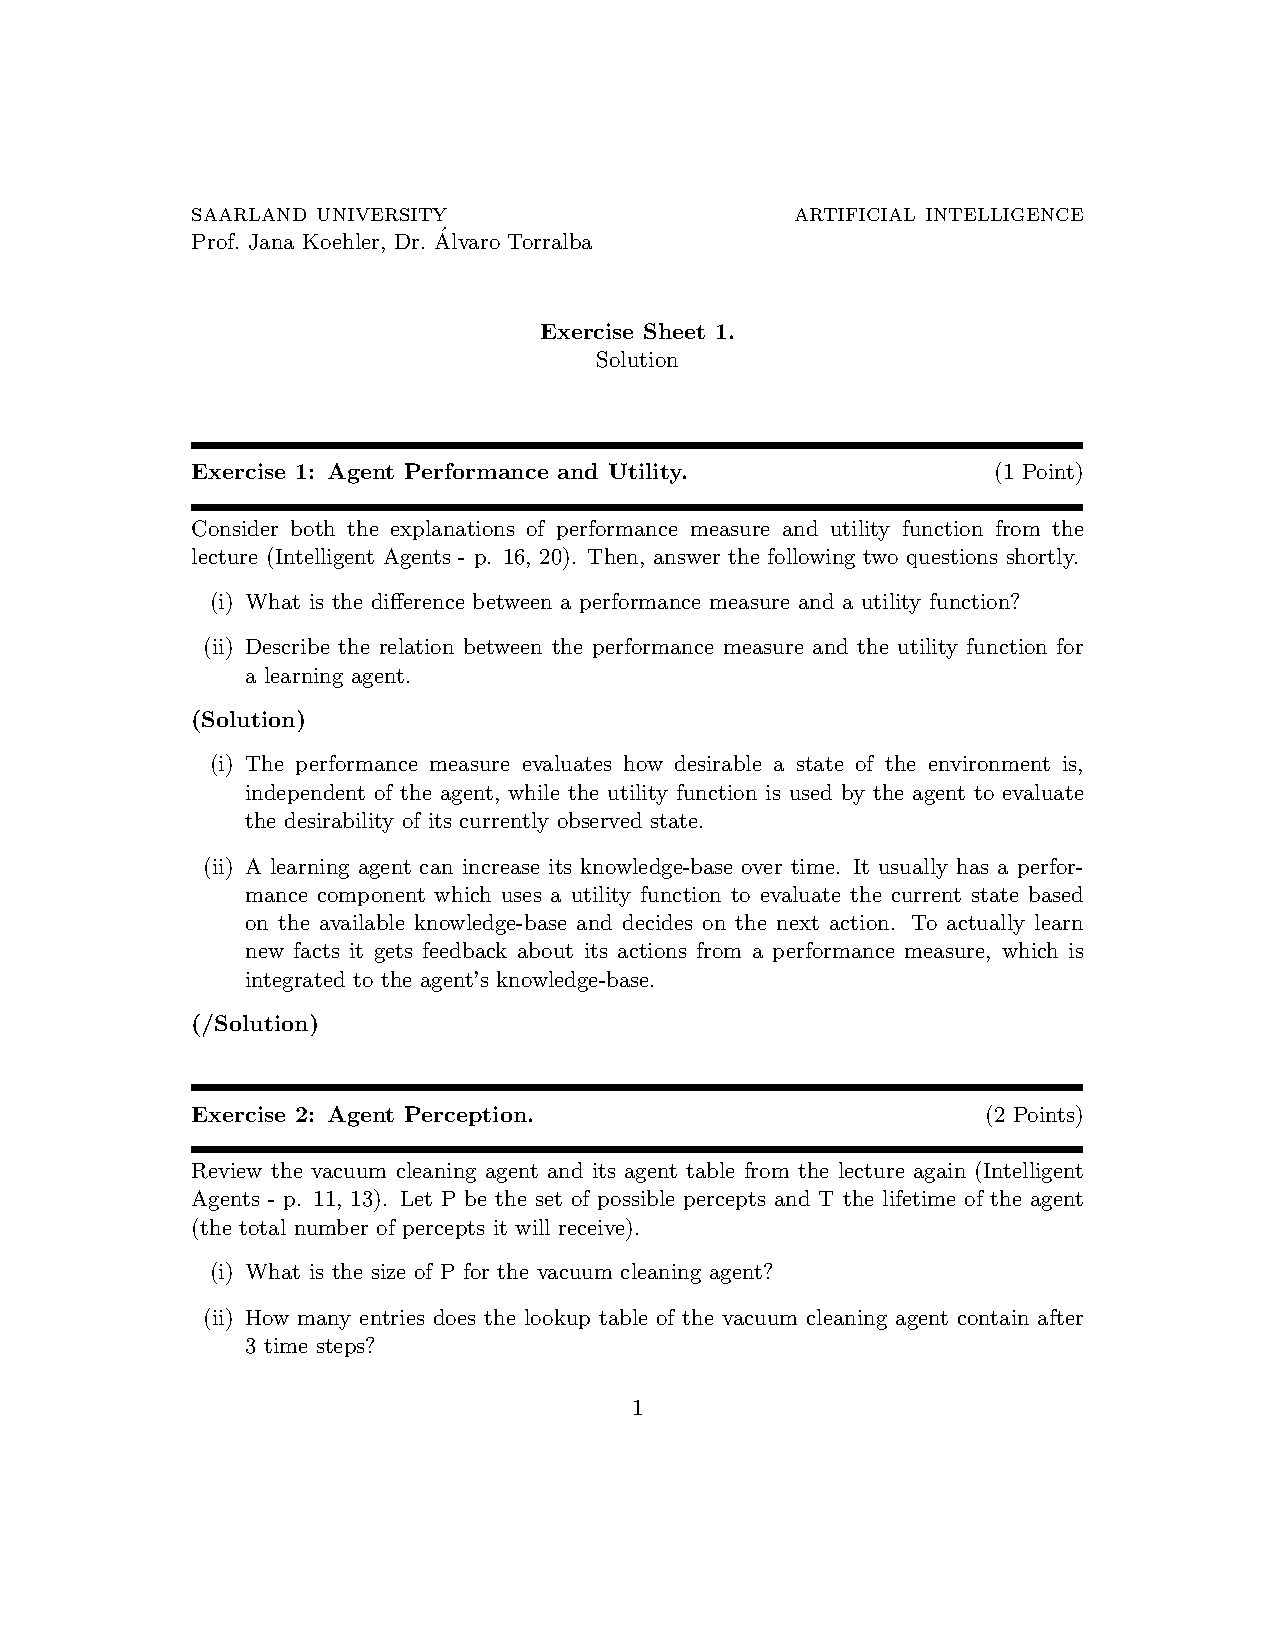
\includepdf[pages=-]{Exercise_Sheet_1_-_Solution.pdf}

\section{Sheet 2}
    \subsection{$A^*$ and Hill Climbing} 
    \subsection{Admissible Heuristics (Vacuum Cleaner, Manhatten Distance)}
    \subsection{DNF}
    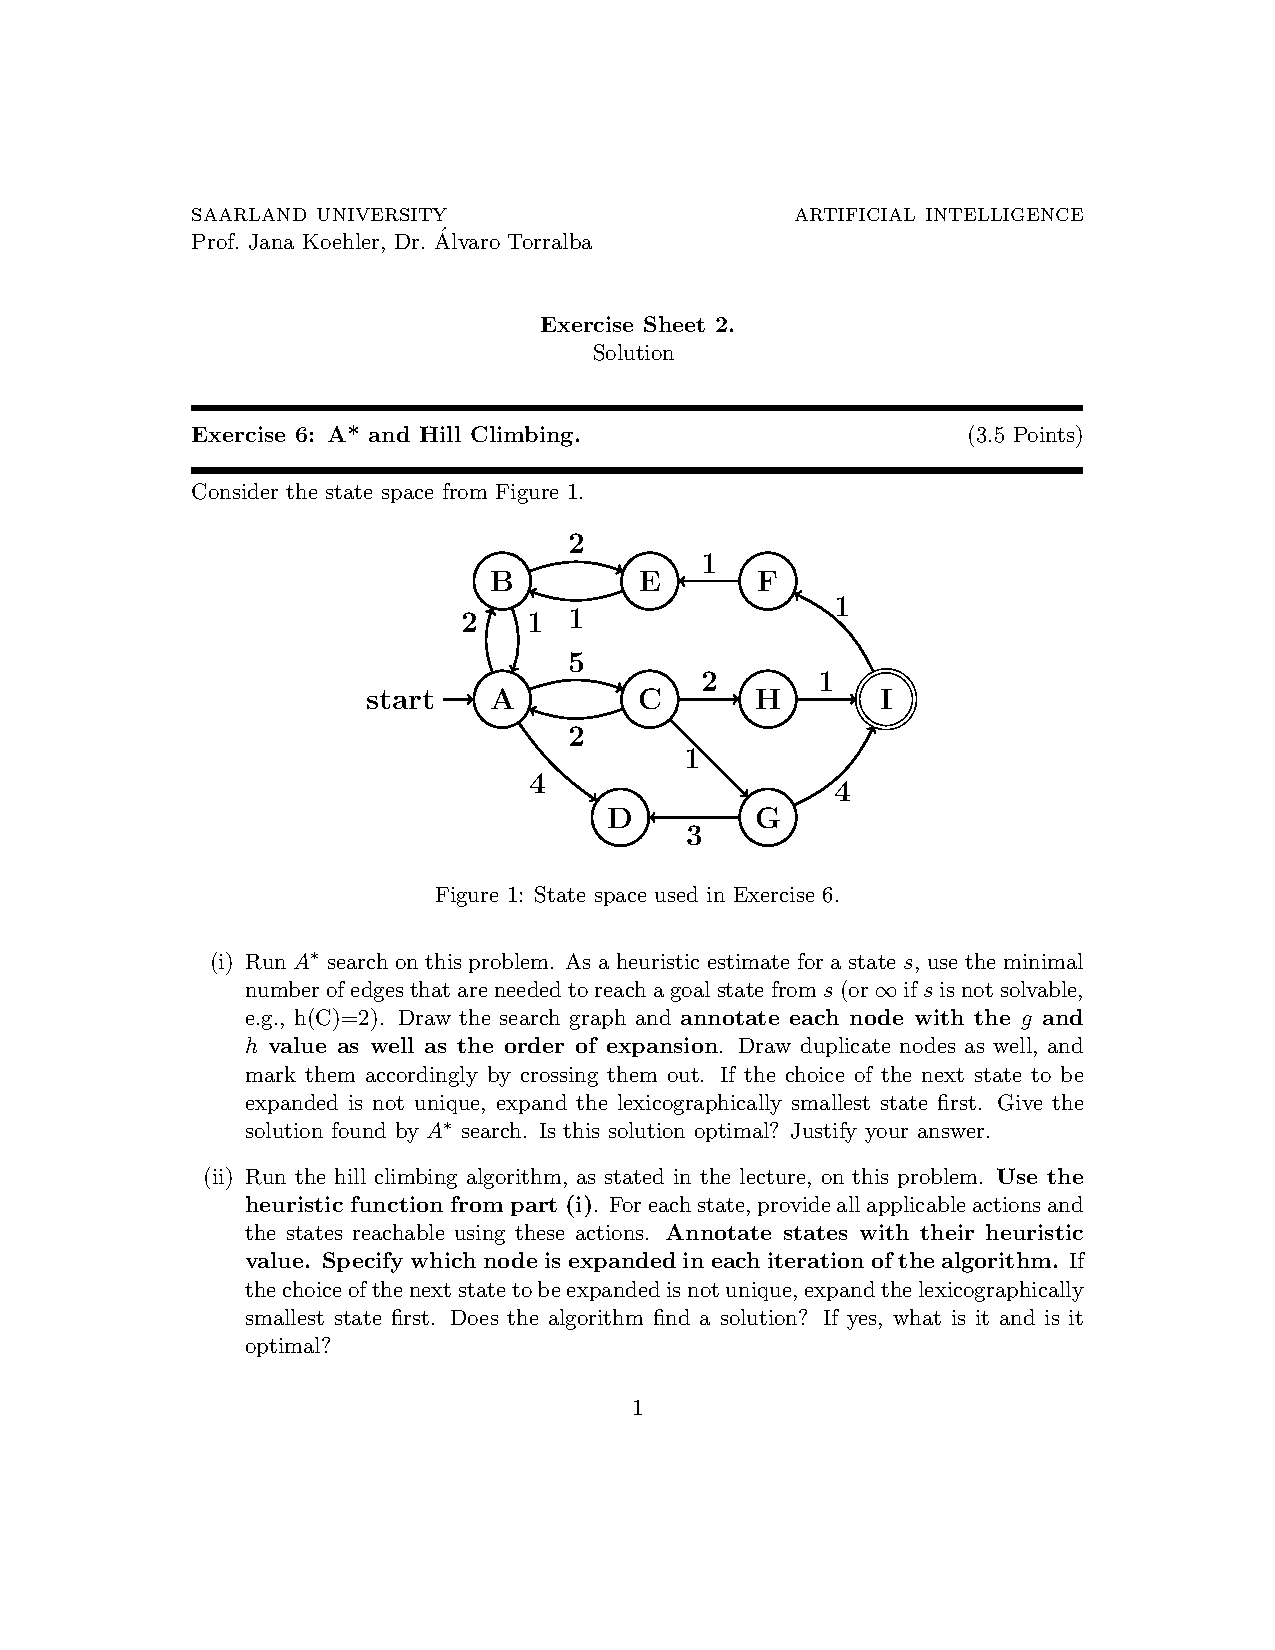
\includepdf[pages=-]{Exercise_Sheet_2_-_Solution.pdf}
    
\section{Sheet 3}
    \subsection{CNF}
    \subsection{Resolution}
    \subsection{DPLL}
    \subsection{CDCL}
    \subsection{Contraposition theorem}
    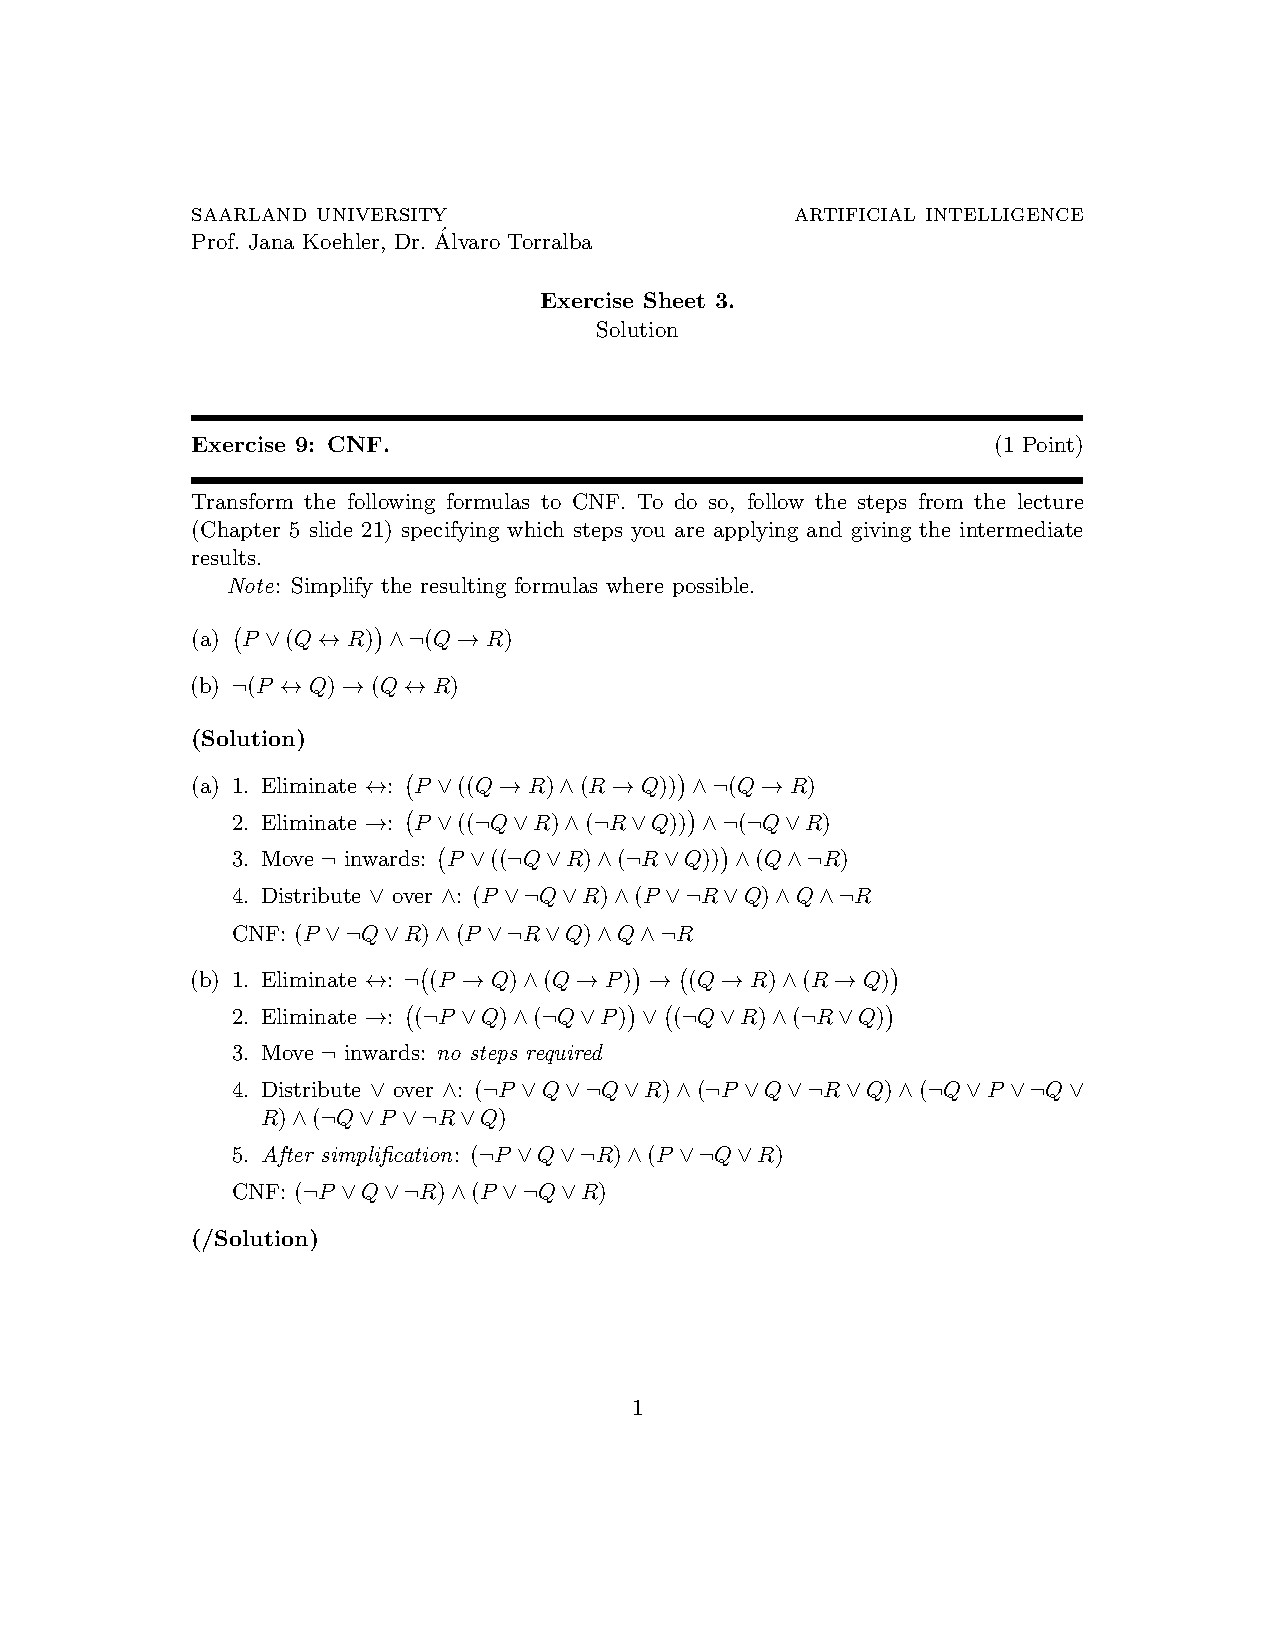
\includepdf[pages=-]{Exercise_Sheet_3_-_Solution.pdf}

\section{Sheet 4}
    \subsection{Predicate Logic Formula}
    \subsection{Predicate  logic  formulas  into  clausal  normal  form}
    \subsection{Herbrand Expansion}
    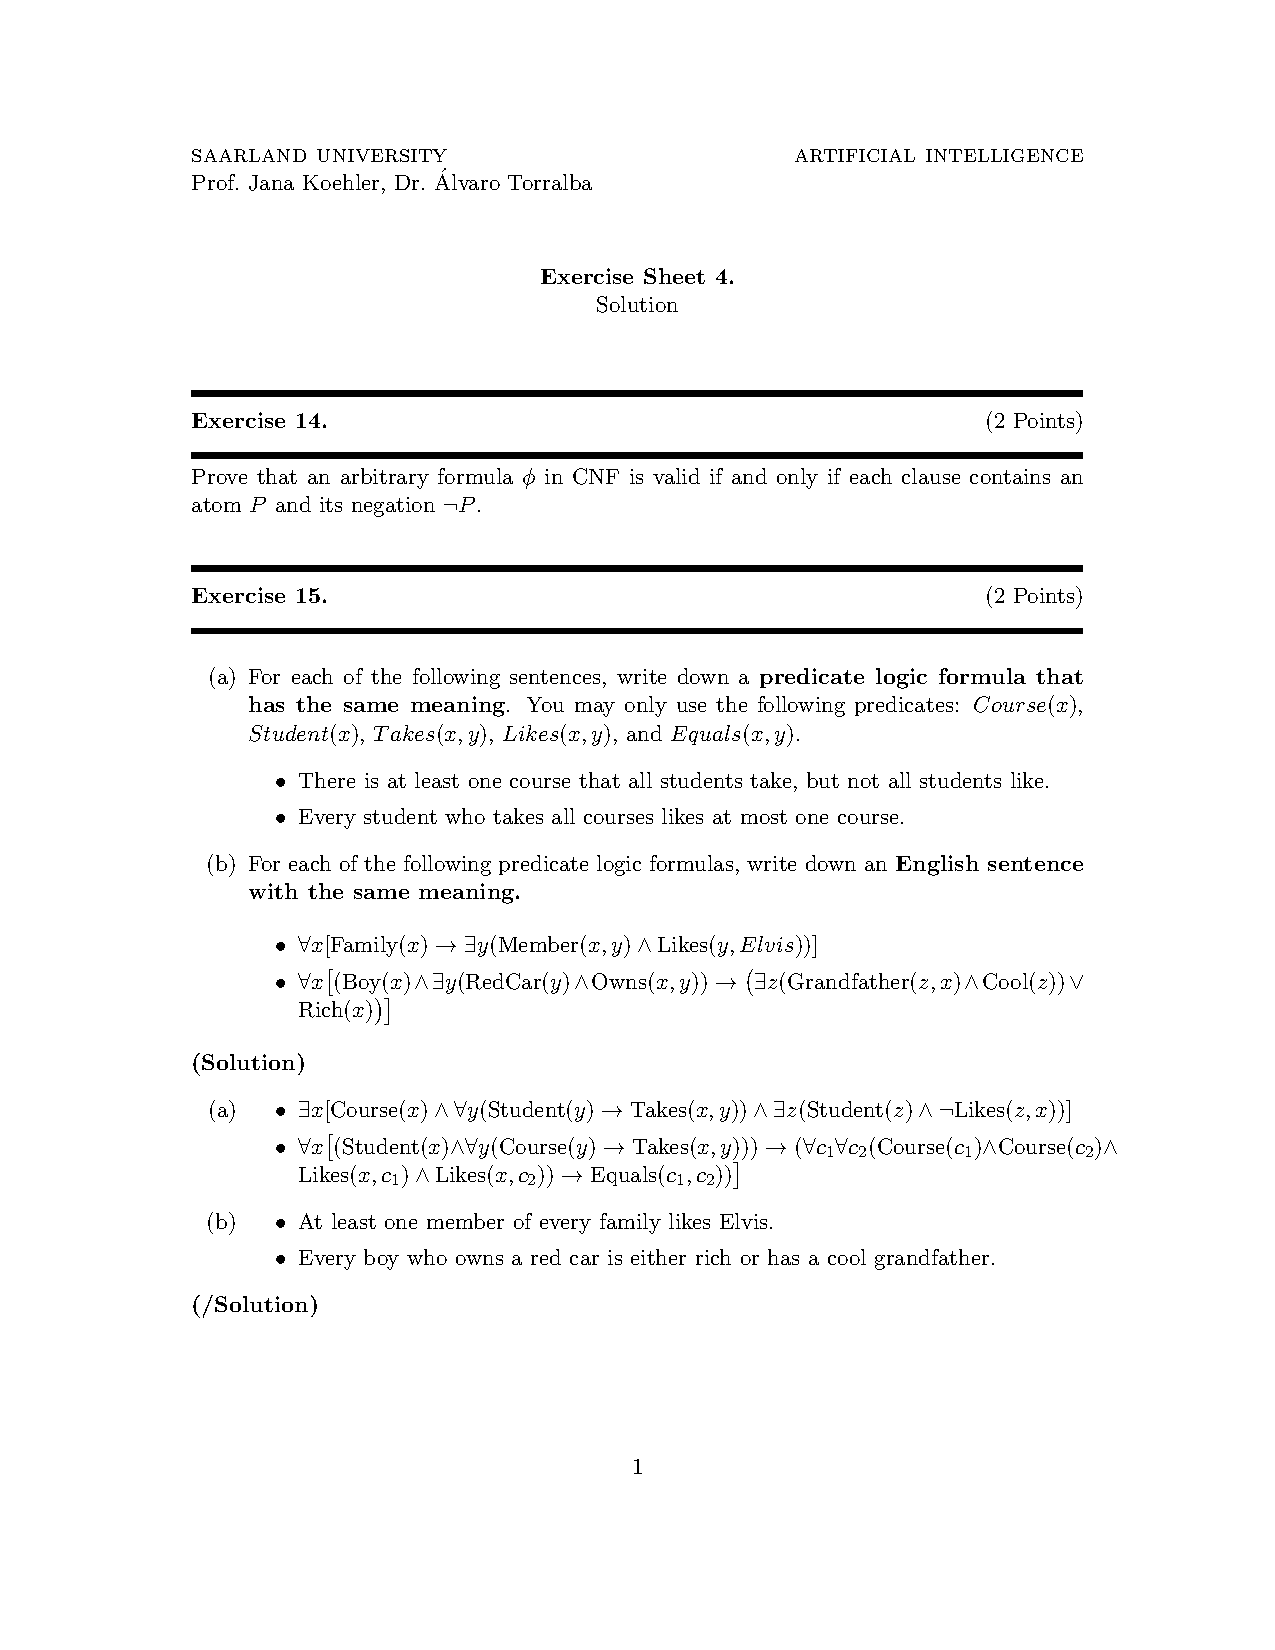
\includepdf[pages=-]{Exercise_Sheet_4_-_Solution.pdf}

\section{Sheet 5}
    \subsection{Unification Algorithm}
    \subsection{PL1 Resolution}
    \subsection{Formulating a constraint network}
    \subsection{Naive backtracking algorithm}
    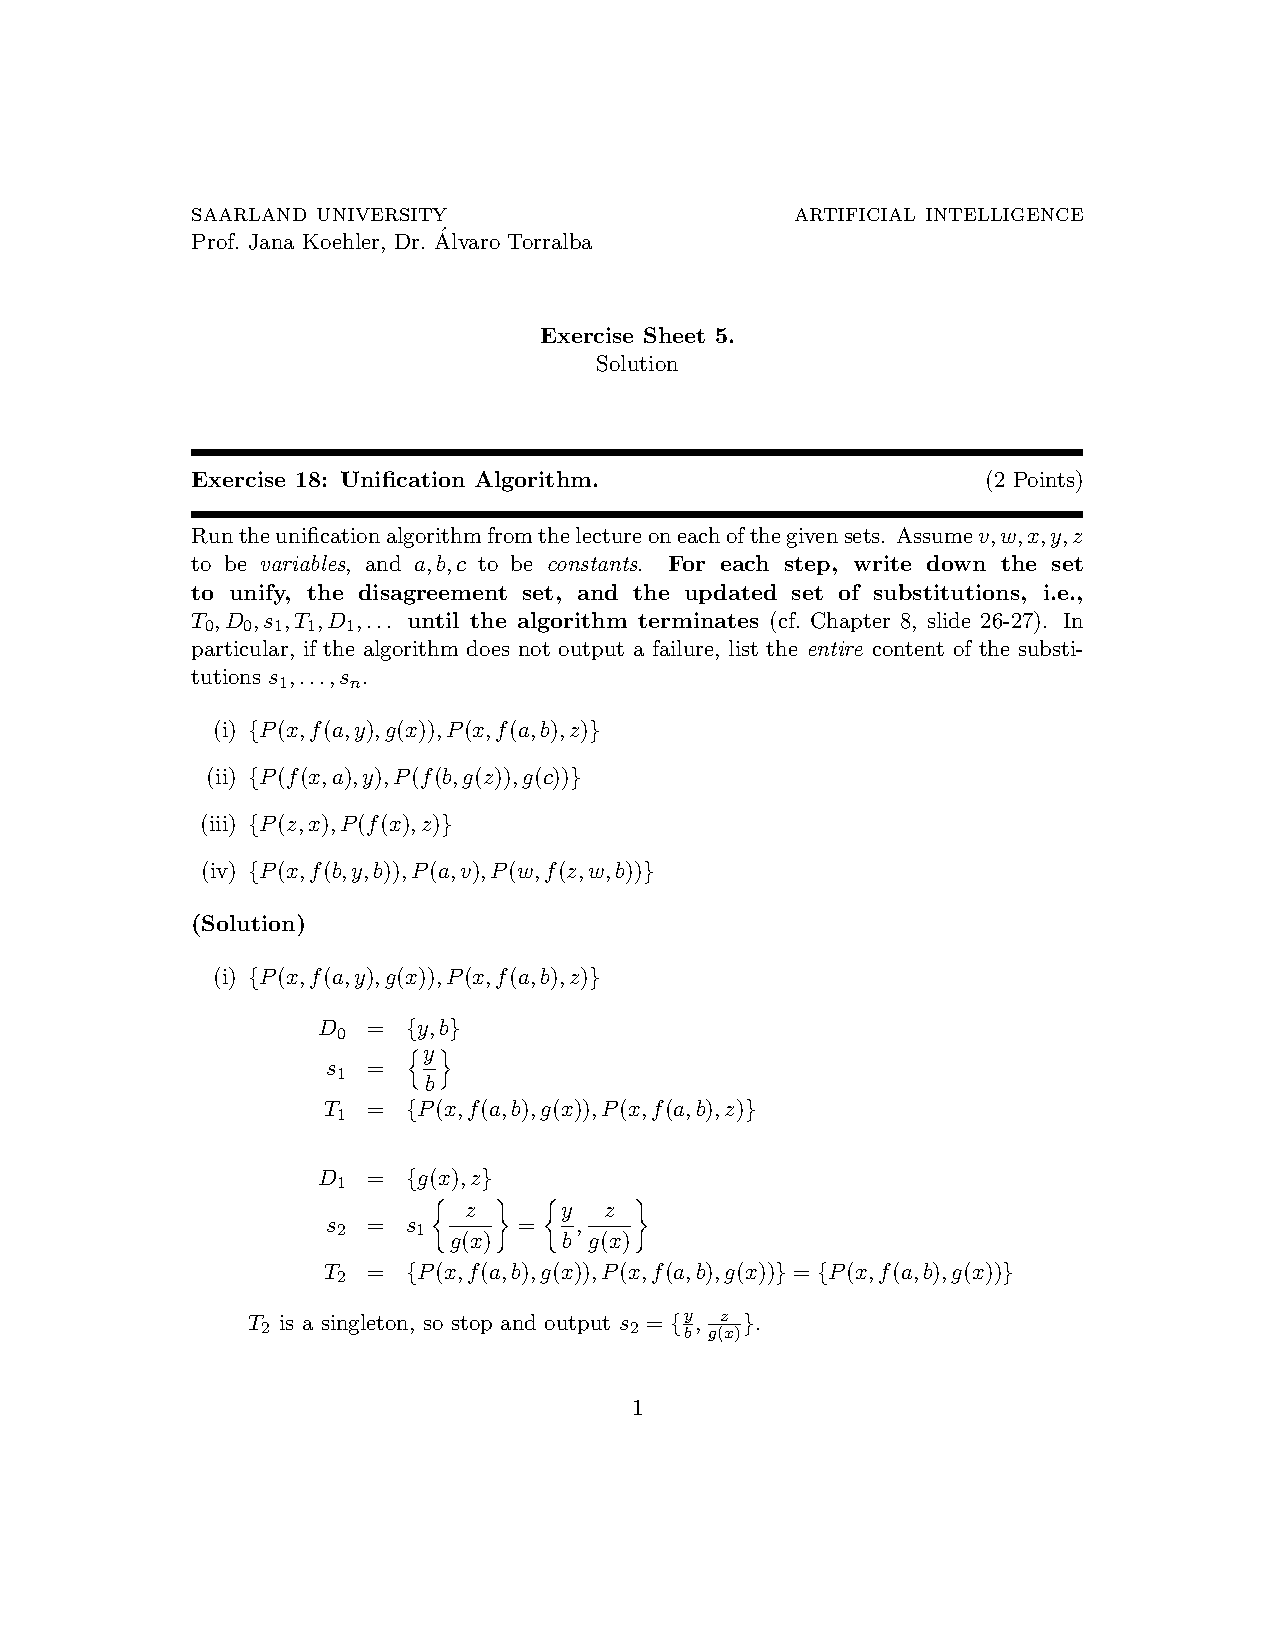
\includepdf[pages=-]{Exercise_Sheet_5_-_Solution.pdf}

\section{Sheet 6}
    \subsection{Constraint Network (AC-3)}
    \subsection{AcyclicCG (BacktrackingWithInference)}
    \subsection{Constraint Network (Draw graph, Cutset)}
    \subsection{Minimax}
    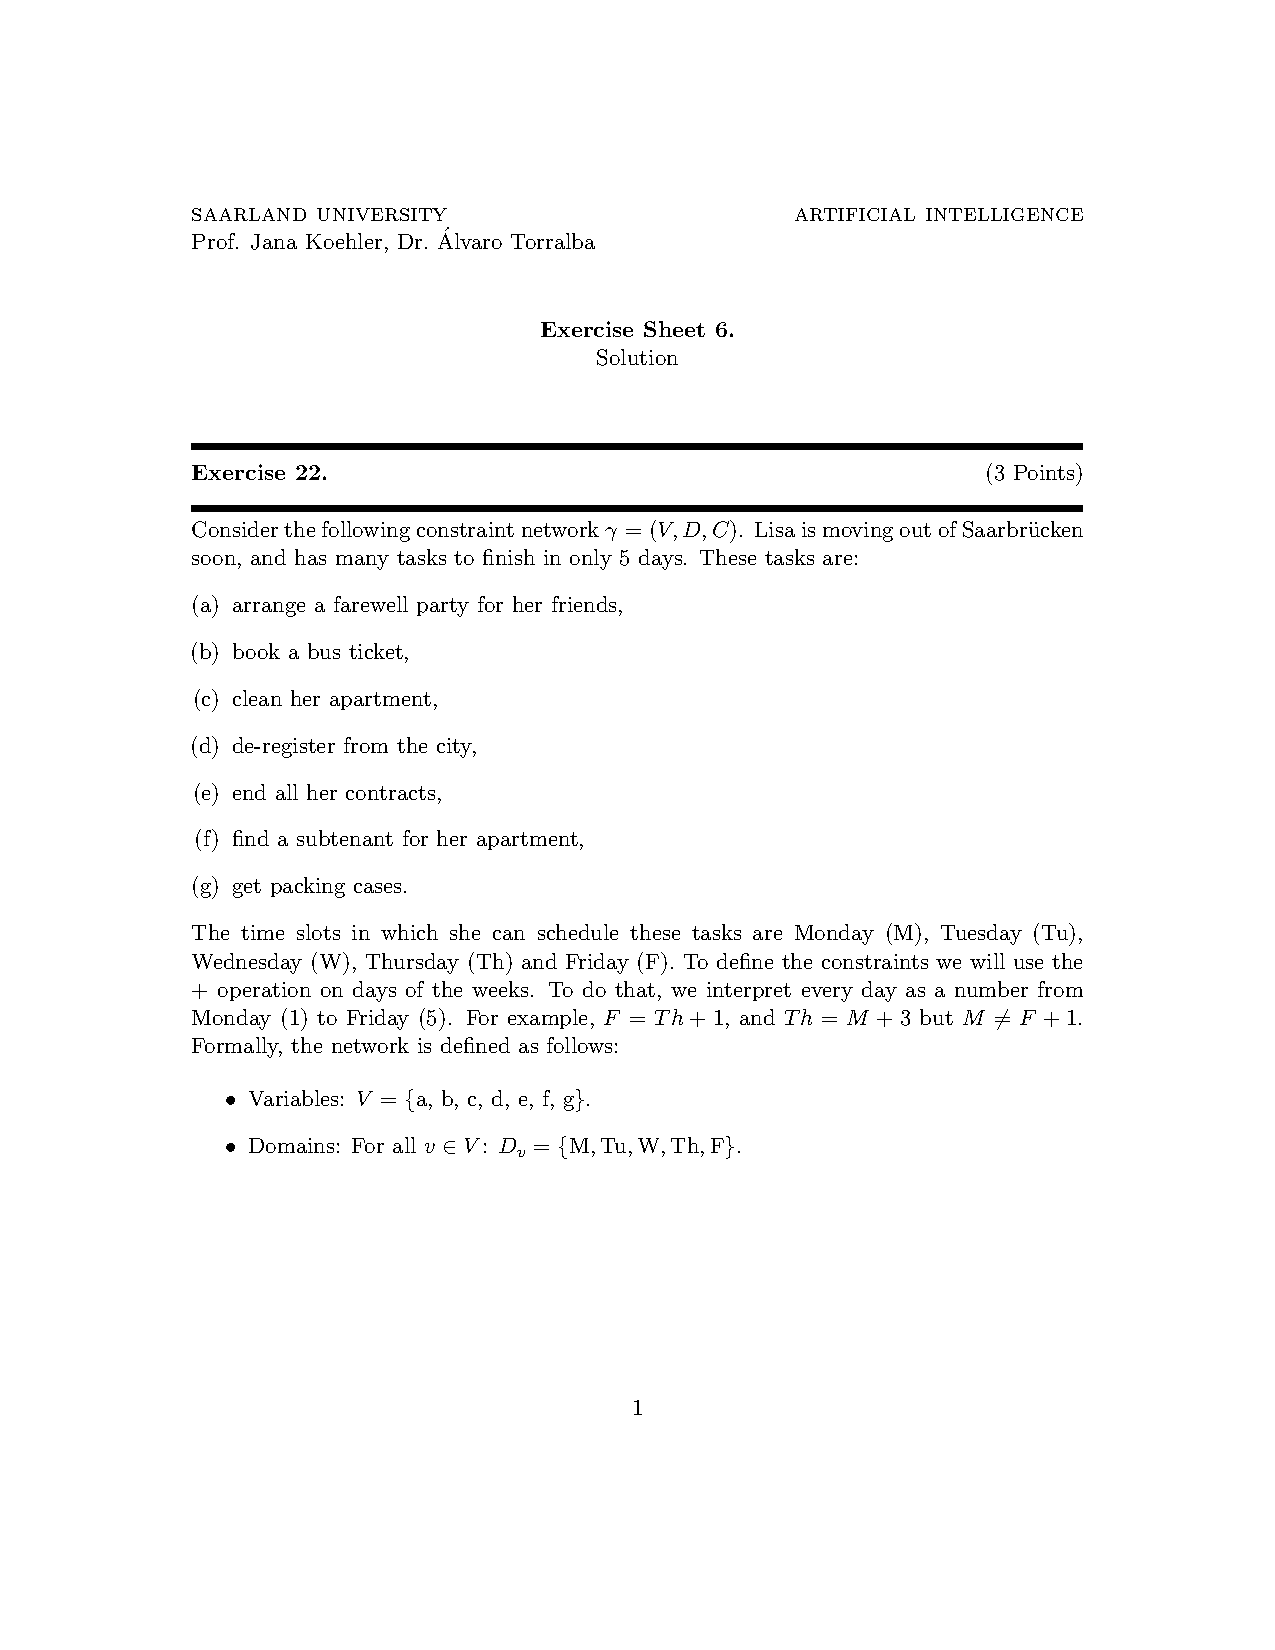
\includepdf[pages=-]{Exercise_Sheet_6_-_Solution.pdf}

\section{Sheet 7}
    \subsection{Alpha-Beta Pruning}
    \subsection{STRIPS}
    \subsection{Planning}
    \subsection{Complexity of Planning}
    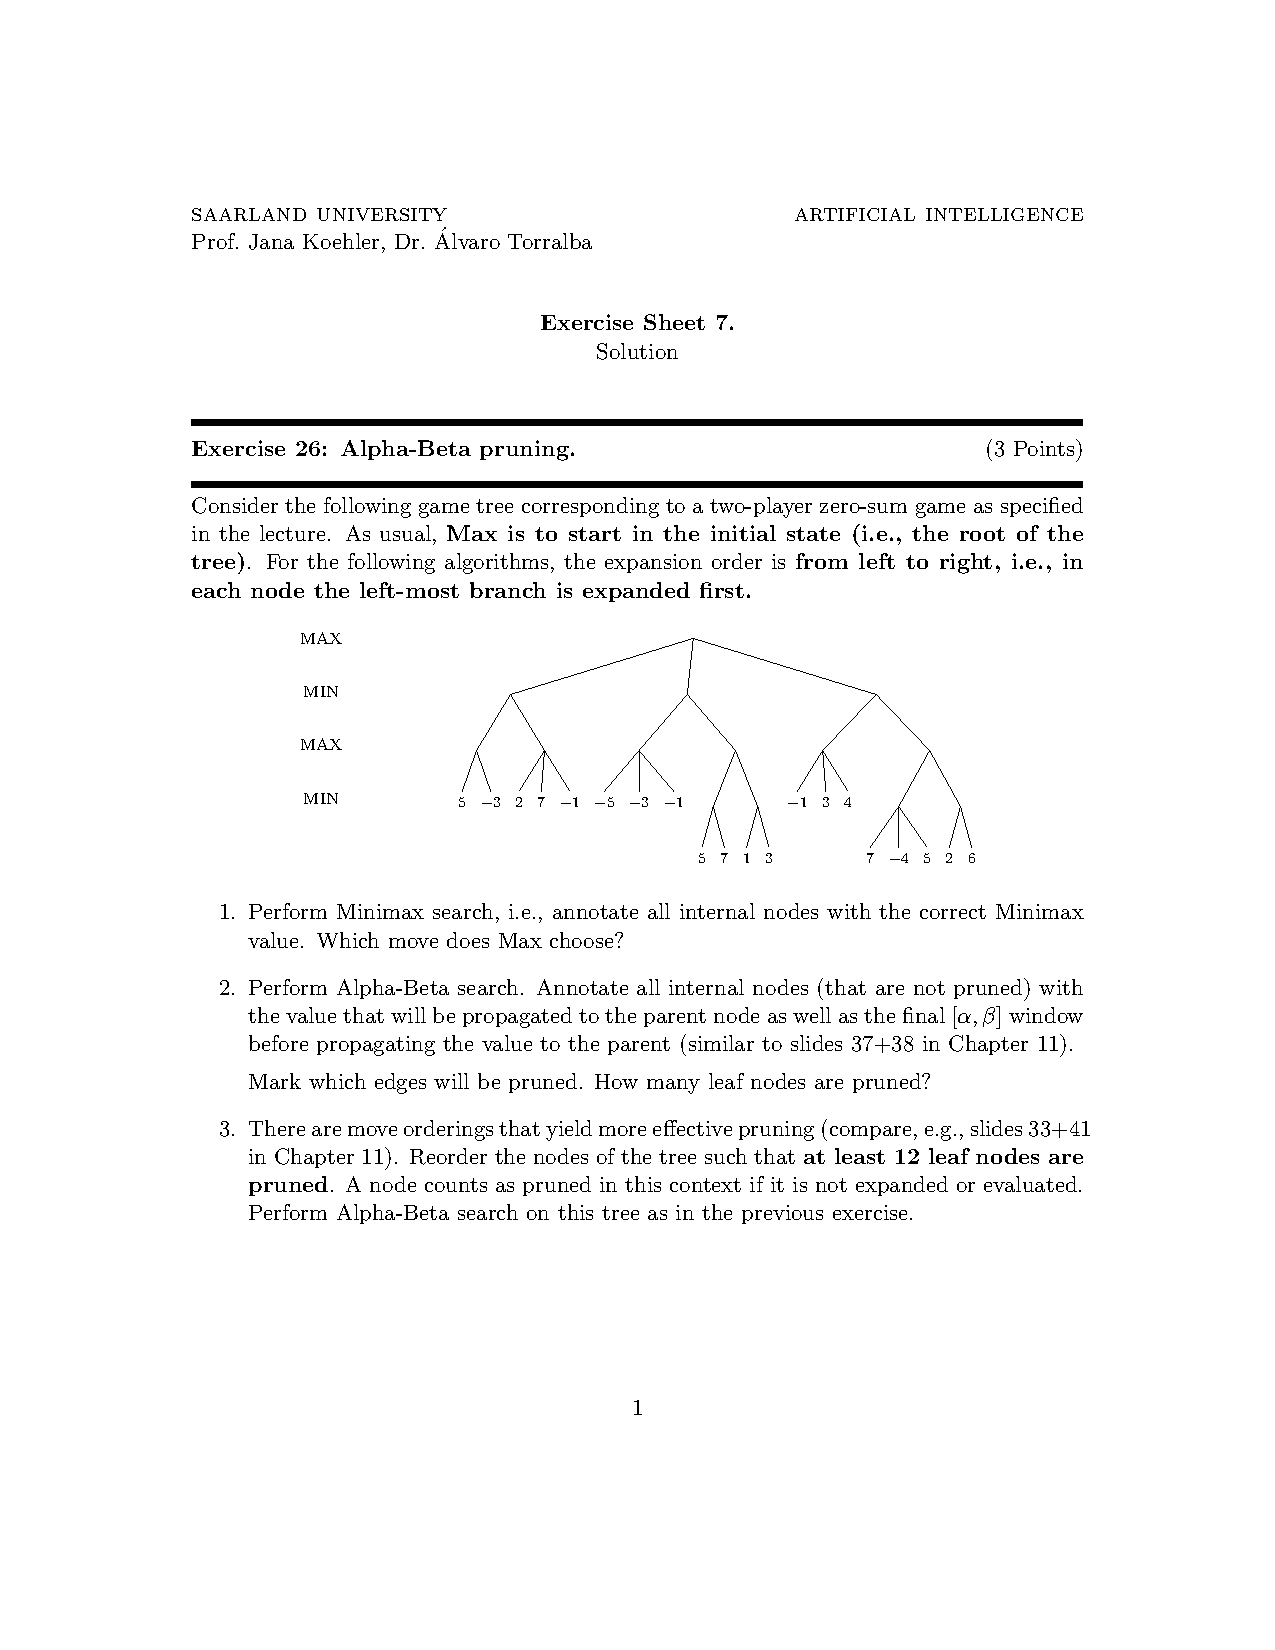
\includepdf[pages=-]{Exercise_Sheet_7_-_Solution.pdf}

\section{Sheet 8}
    \subsection{Delete relaxation – Search with $h^+$}
    \subsection{Delete relaxation - $h^{max},h^{FF}$}
    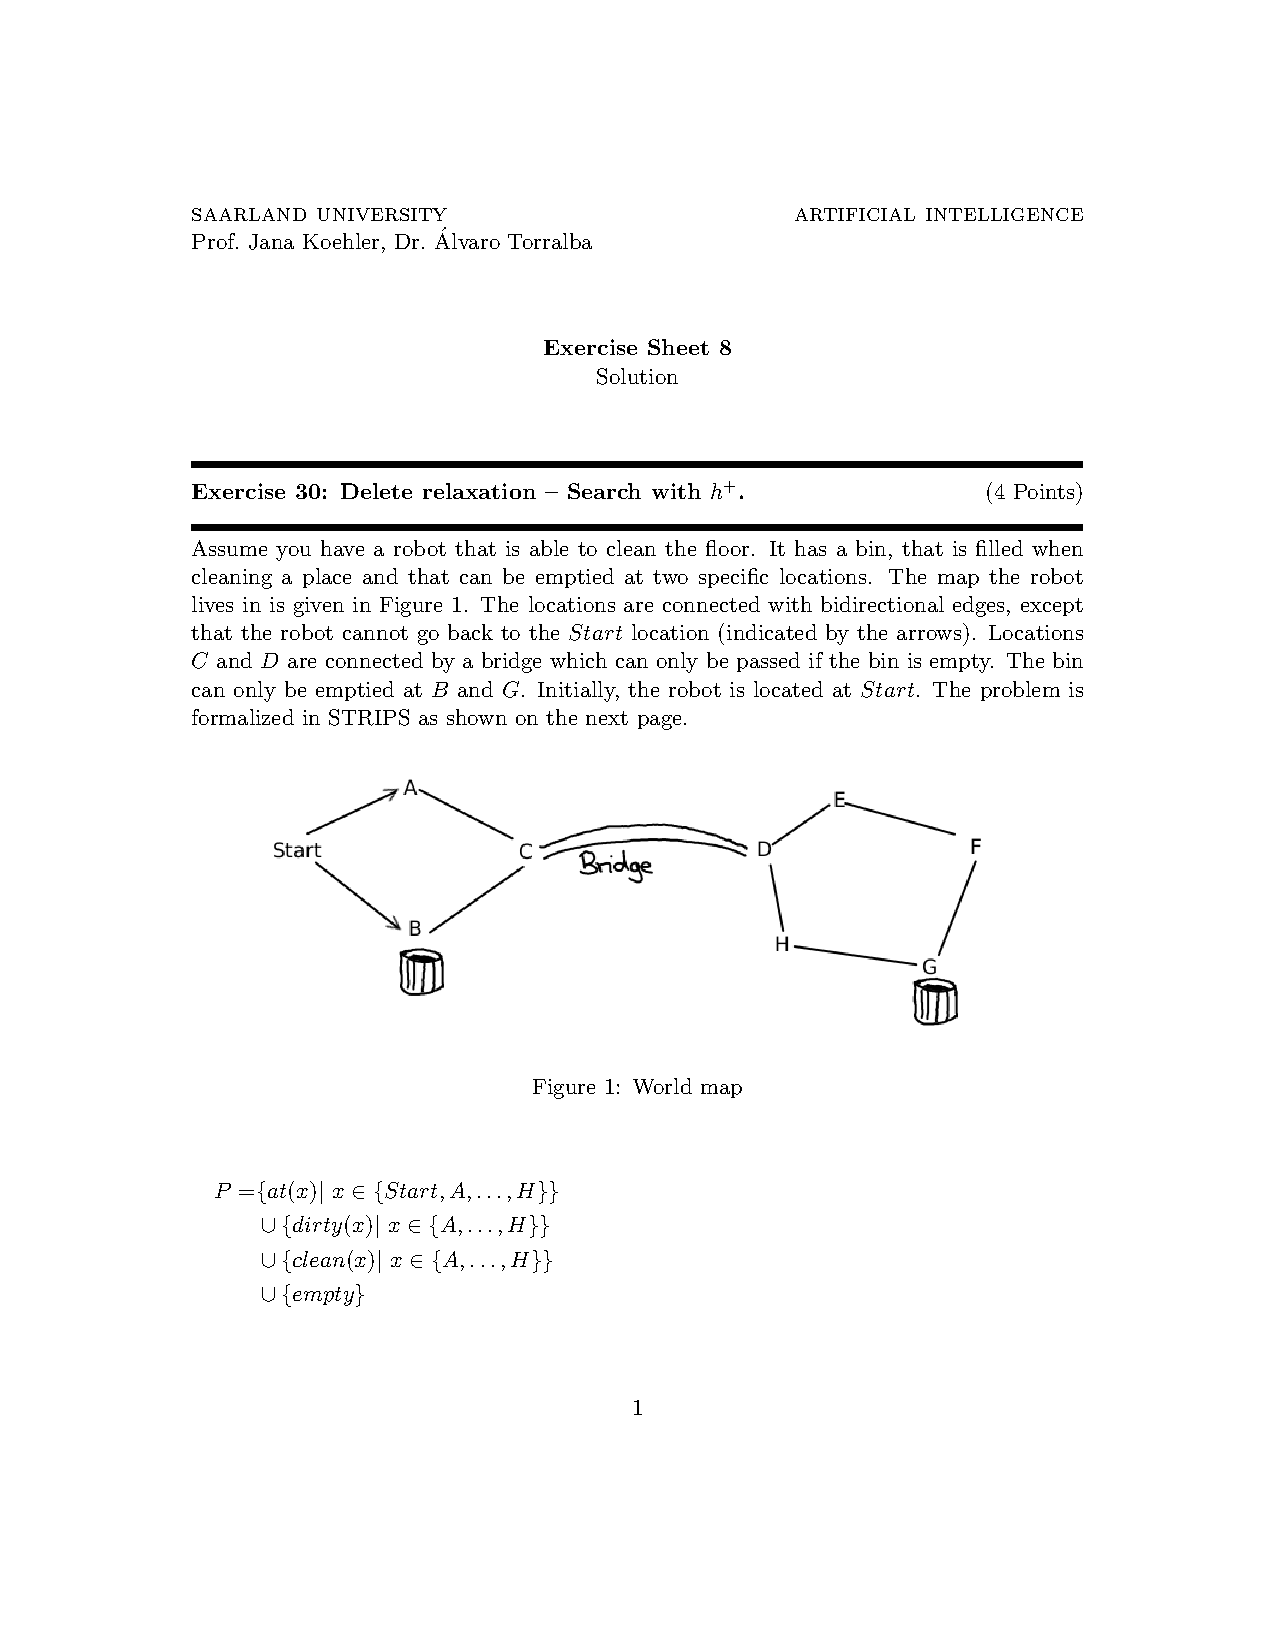
\includepdf[pages=-]{Exercise_Sheet_8_-_Solution.pdf}

\section{Sheet 9}
    \subsection{Probability Theory}
    \subsection{Probability Theory}
    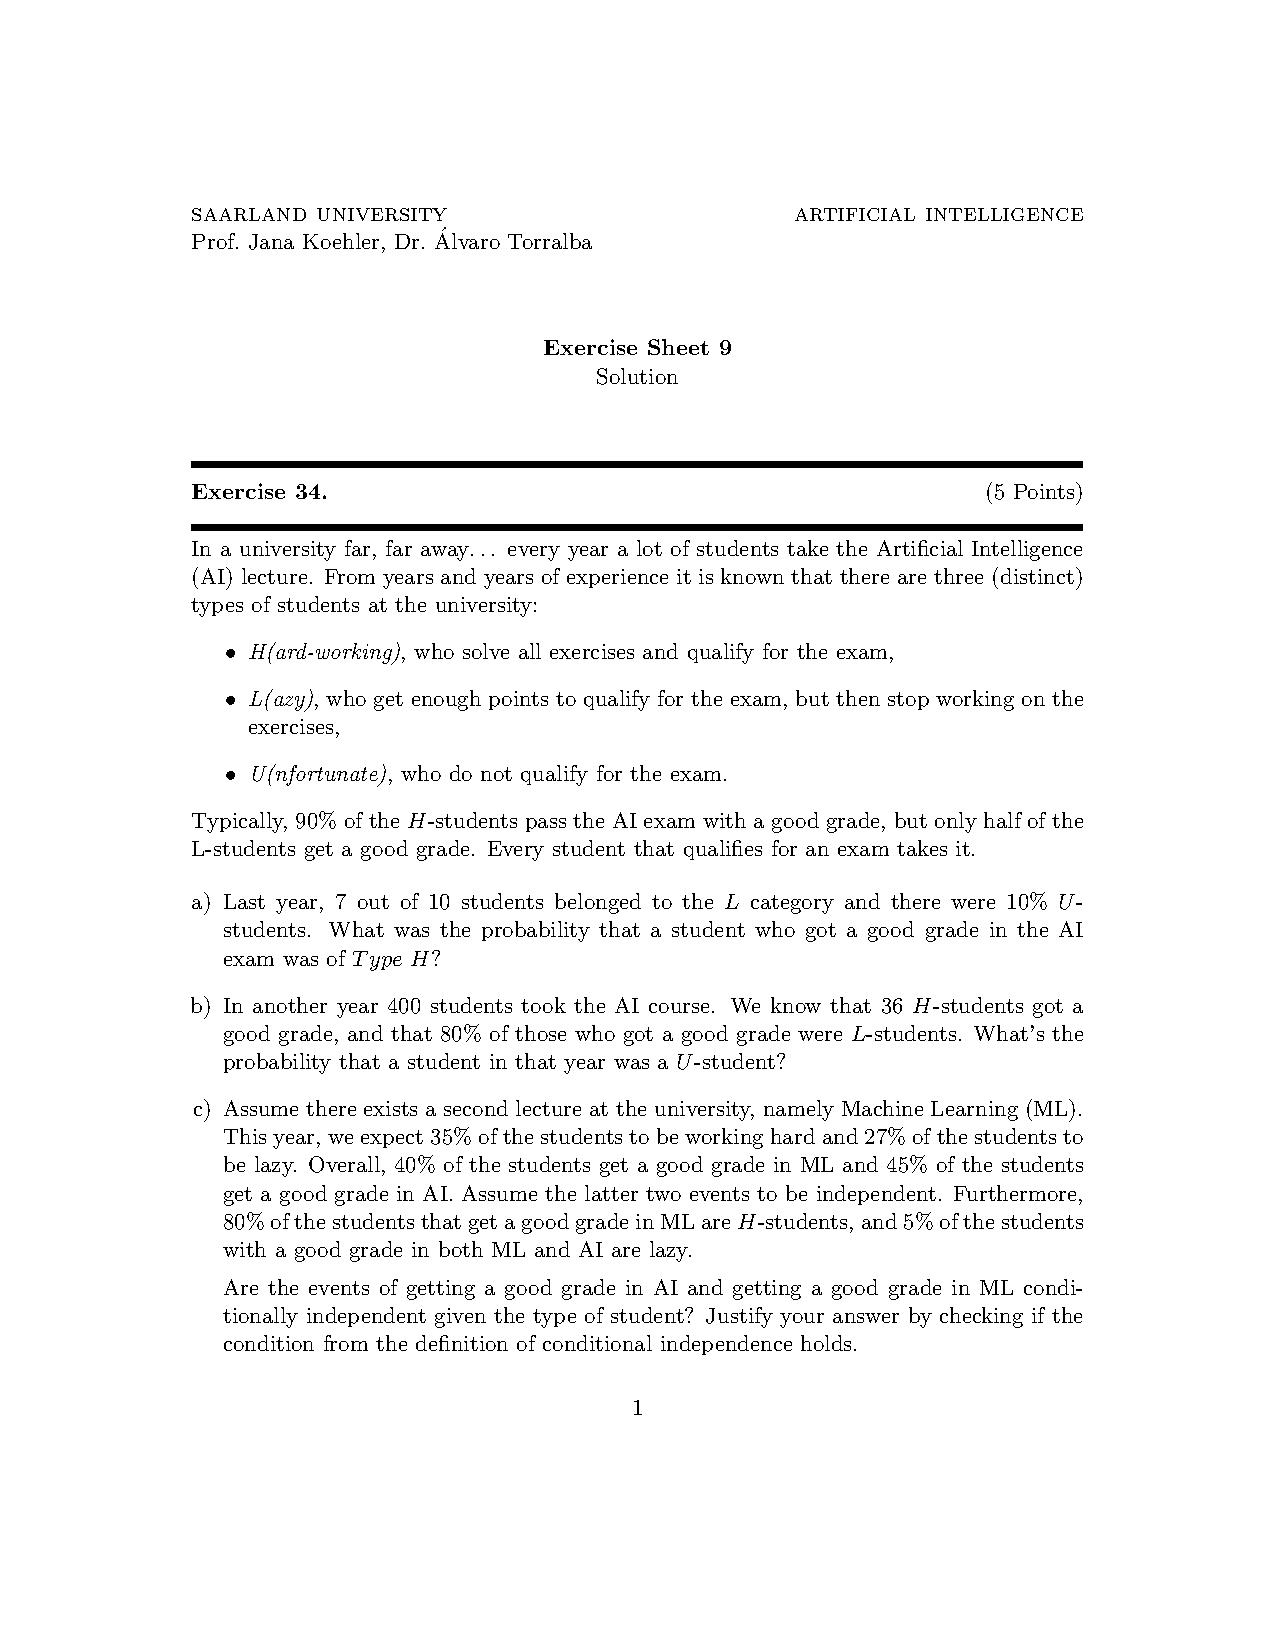
\includepdf[pages=-]{Exercise_Sheet_9_-_Solution.pdf}

\section{Sheet 10}
    \subsection{Bayesian inference}
    \subsection{Construction of Bayesian networks}
    \subsection{$\mathcal{ALC}$}
    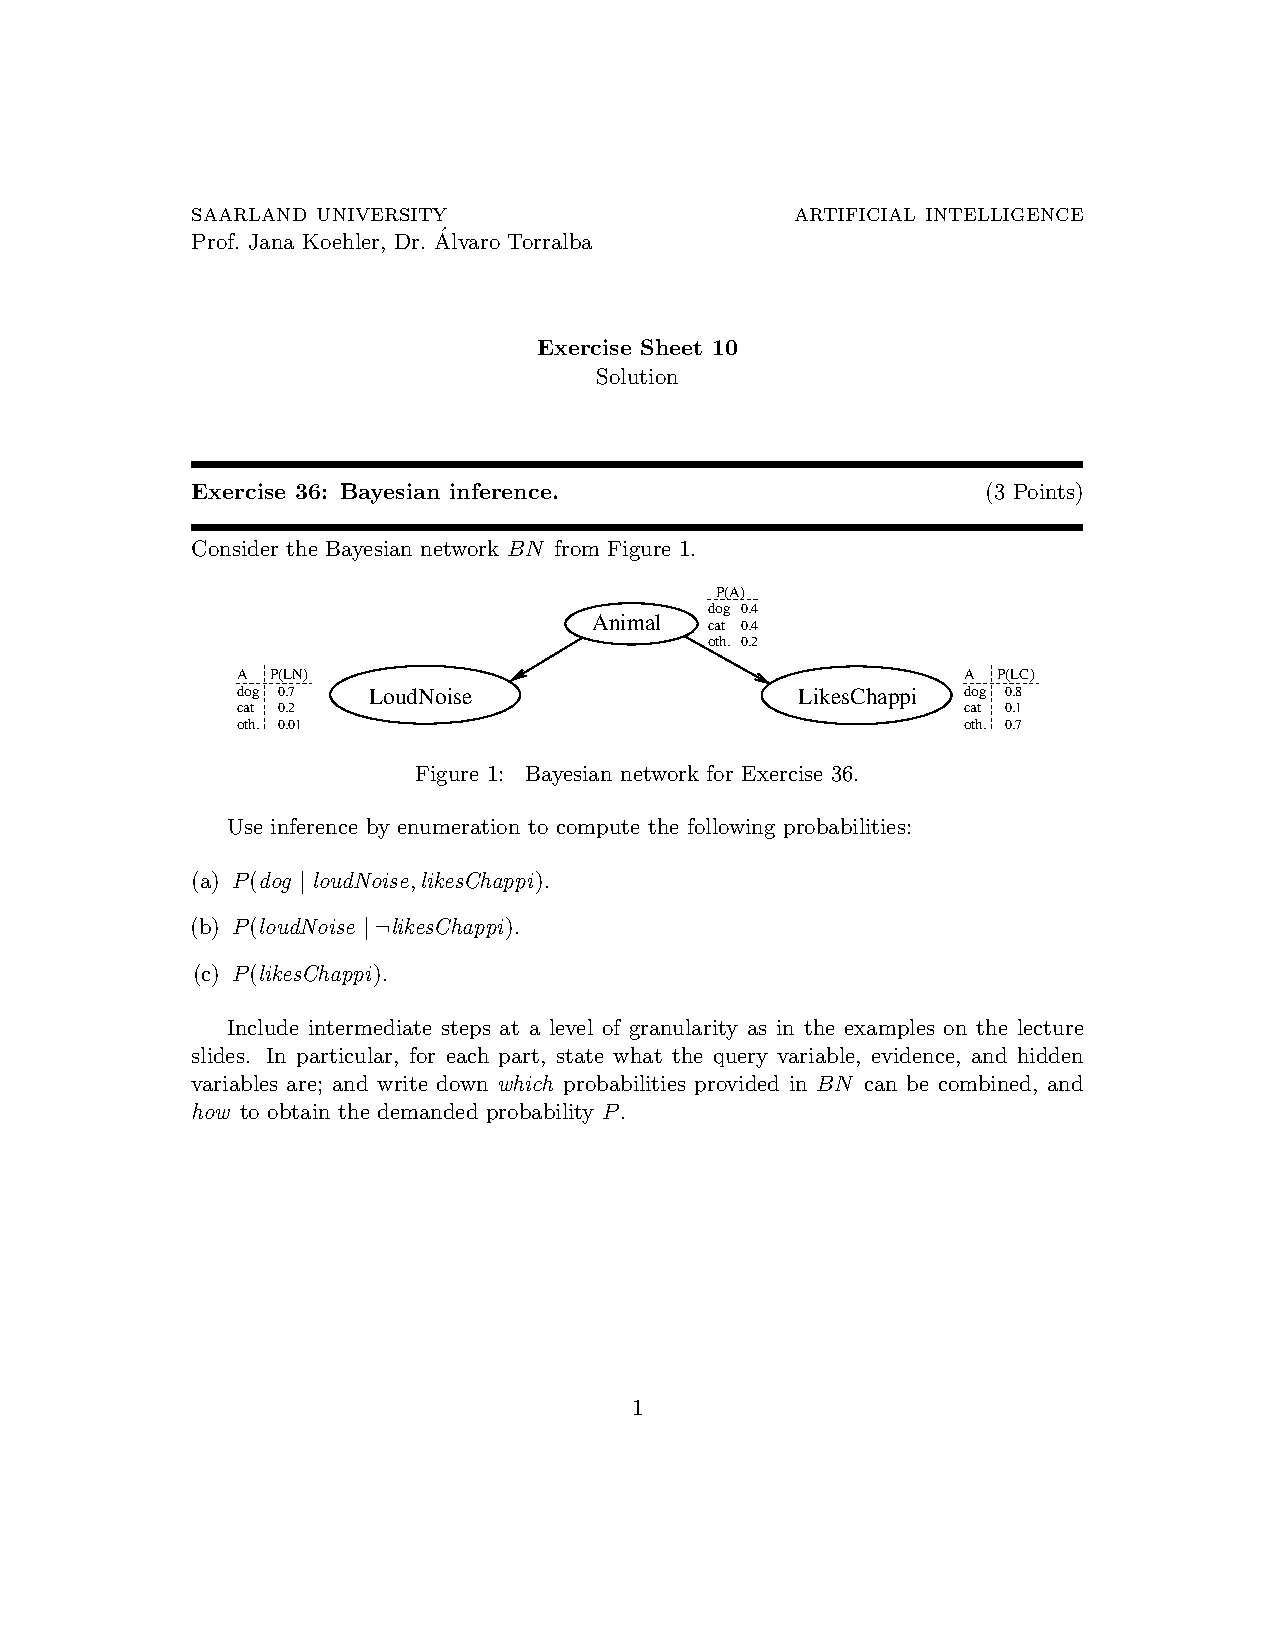
\includepdf[pages=-]{Exercise_Sheet_10_-_Solution.pdf}



\section{AI 2016}
    \subsection{Sheet 1:}
        \subsubsection{Exercise 1: UCS, $A^*$, Hill Climbing algorithm, Heuristic, Iterative DFS}
        \subsubsection{Exercise 2: Vacuum Cleaner (Heuristic), }
        \subsubsection{Exercise 3: DFS, Iterative-Deepening search}
    \subsection{Sheet 2:}
        \subsubsection{Exercise 4: Tic-Tac-Toe (Minimax), Evaluation Function}
        \subsubsection{Exercise 5: Minimax search, Alpha-Beta search, Pruning}
        \subsubsection{Exercise 6: Naive Backtracking, Variable Ordering}
        \subsubsection{Exercise 7: Crossword Puzzle, Specify variable domains and constraints}
    \subsection{Sheet 3:}
        \subsubsection{Exercise 8: Naive Backtracking, Constraint Network, CSP Problem}
        \subsubsection{Exercise 9: Constraint Network, AC-3}
        \subsubsection{Exercise 10: Constraint Network, AcyclicCG, BacktrackingWithInference}
        \subsubsection{Exercise 11: Constraint Network, Optimal (minimal) Cutset, Cutset Conditioning algorithm, AcyclicCG}
    \subsection{Sheet 4:}
        \subsubsection{Exercise 13: Transform to CNF}
        \subsubsection{Exercise 14: Use resolution that CNF formulas are unsatisfiable}
        \subsubsection{Exercise 15: DPLL}
\newpage
    \subsection{Sheet 5:}
        \subsubsection{Exercise 18: DPLL with clause learning}
        \subsubsection{Exercise 19: Predicate Logic Formula}
        \subsubsection{Exercise 20: Transform Predicate Logic Formulas into Clausal Normal Form}
    \subsection{Sheet 6:}
        \subsubsection{Exercise 21: Unification algorithm}
        \subsubsection{Exercise 22: Predicate Logic Formulas in Skolem Normal Form}
        \subsubsection{Exercise 23: Skolem Normal Form, Clausal Normal Form, Binary PL1 Resolution}
    \subsection{Sheet 7:}
        \subsubsection{Exercise 25: Planning Task, STRIPS formalization}
        \subsubsection{Exercise 26: Planning Task, STRIPS formalization}
        \subsubsection{Exercise 27: Planning Task, STRIPS formalization, road map, search on tree}
    \subsection{Sheet 8:}
        \subsubsection{Exercise 29: Blocksworld Problem, $h^{FF}$, $A^*$, $h^+$}
        \subsubsection{Exercise 30: Blocksworld problem, STRIPS, $h^{add}$}
    \subsection{Sheet 9:}
        \subsubsection{Exercise 1: Model an Indoor Soccer-Team Ontology in RDF}
        \subsubsection{Exercise 2: Taxonomy}
        \subsubsection{Exercise 3: Roles}
    \subsection{Sheet 10:}
        \subsubsection{Exercise 1: OWL - Preparation}
        \subsubsection{Exercise 2: OWL - Ontology Browsing}
        \subsubsection{Exercise 3: Production Systems}
    
        
    
    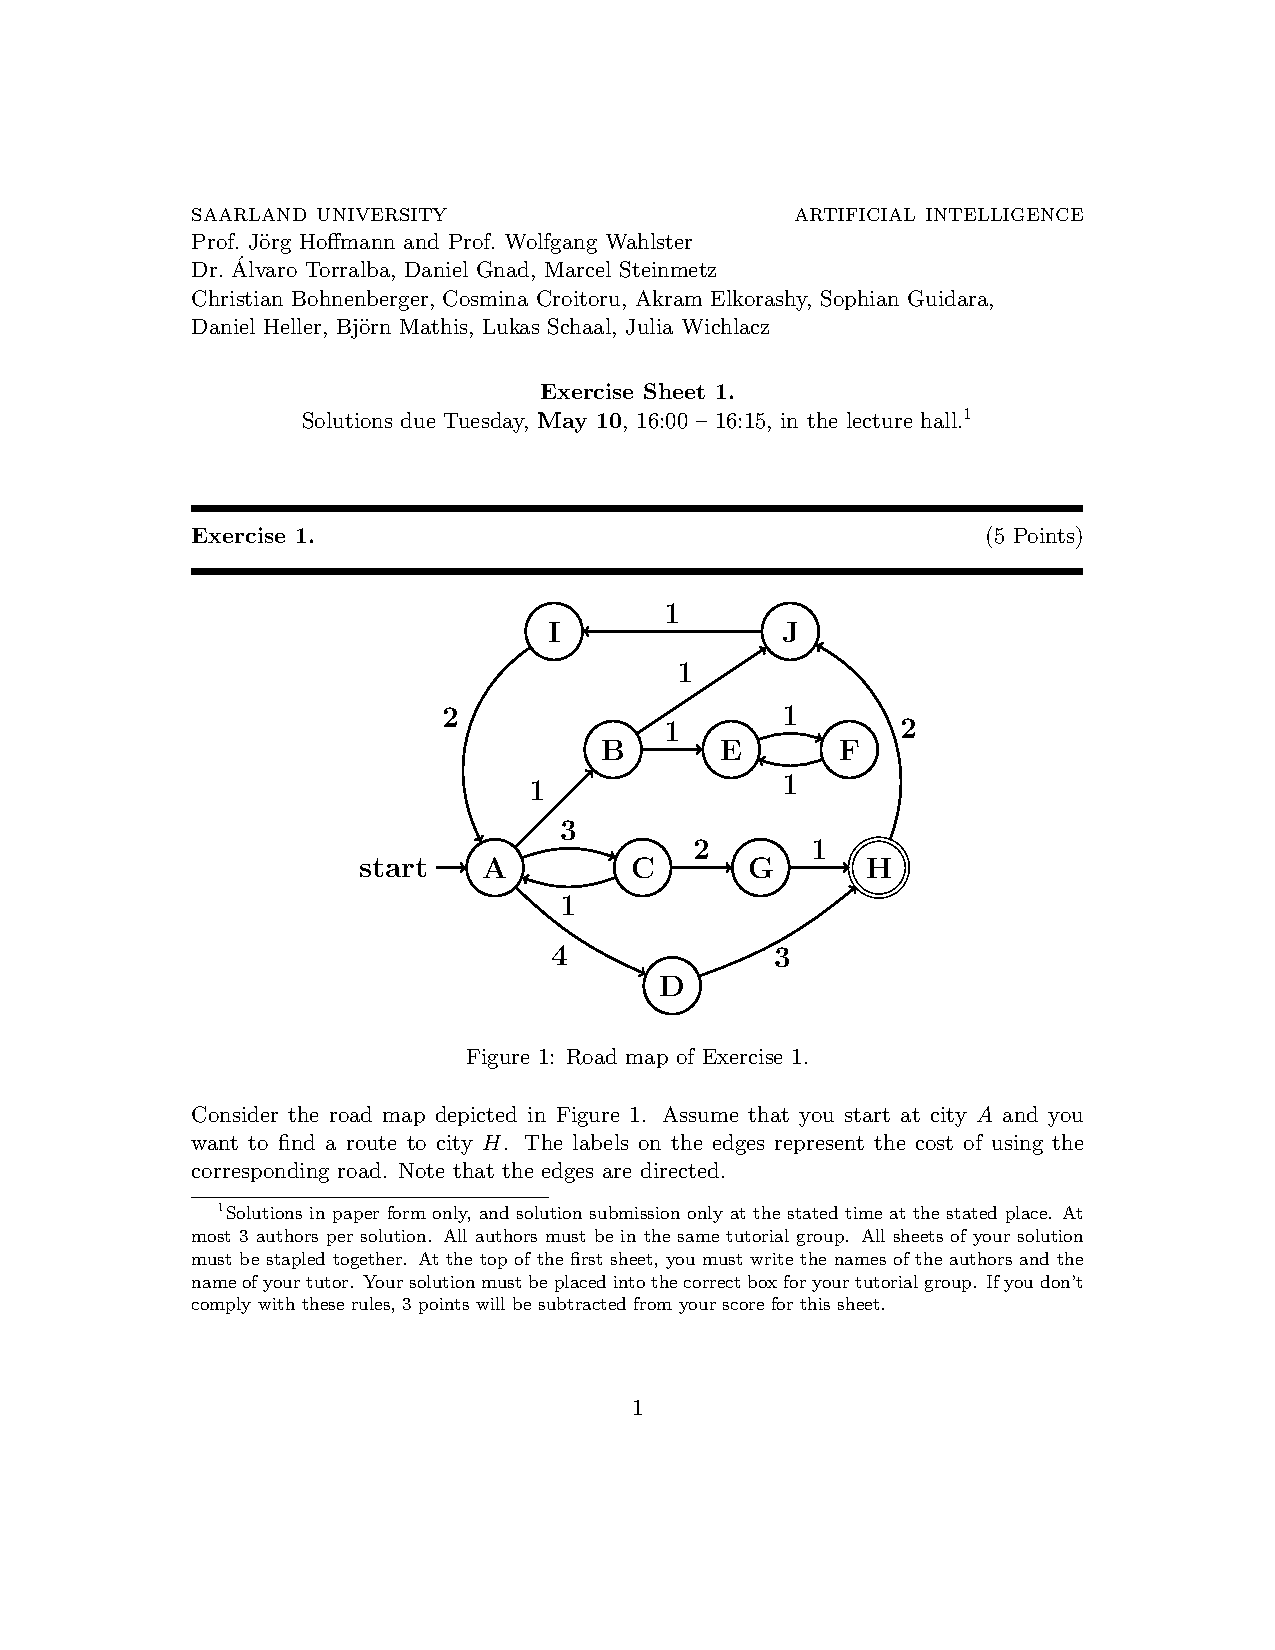
\includepdf[pages=-,nup=2x2]{Old/ai16_sheet01_solution.pdf}
    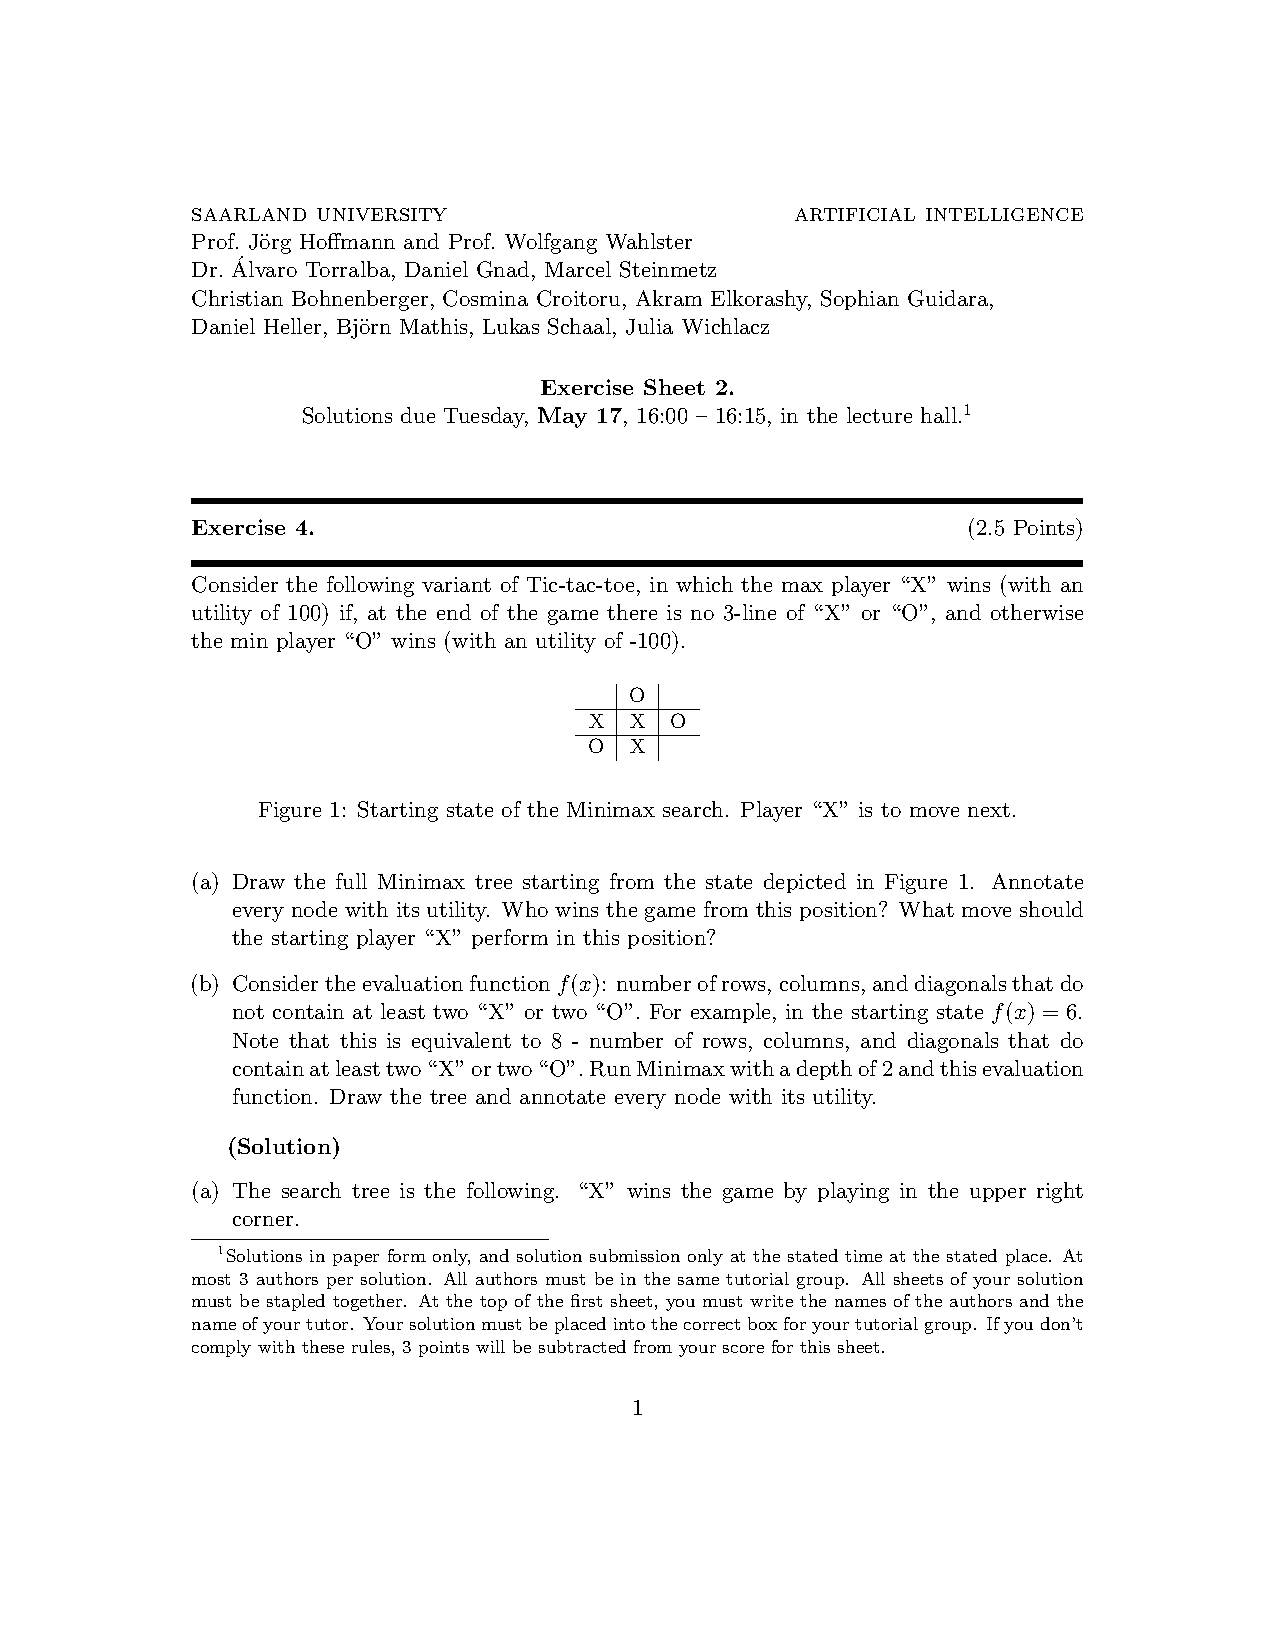
\includepdf[pages=-,nup=2x2]{Old/ai16_sheet02_solution.pdf}
    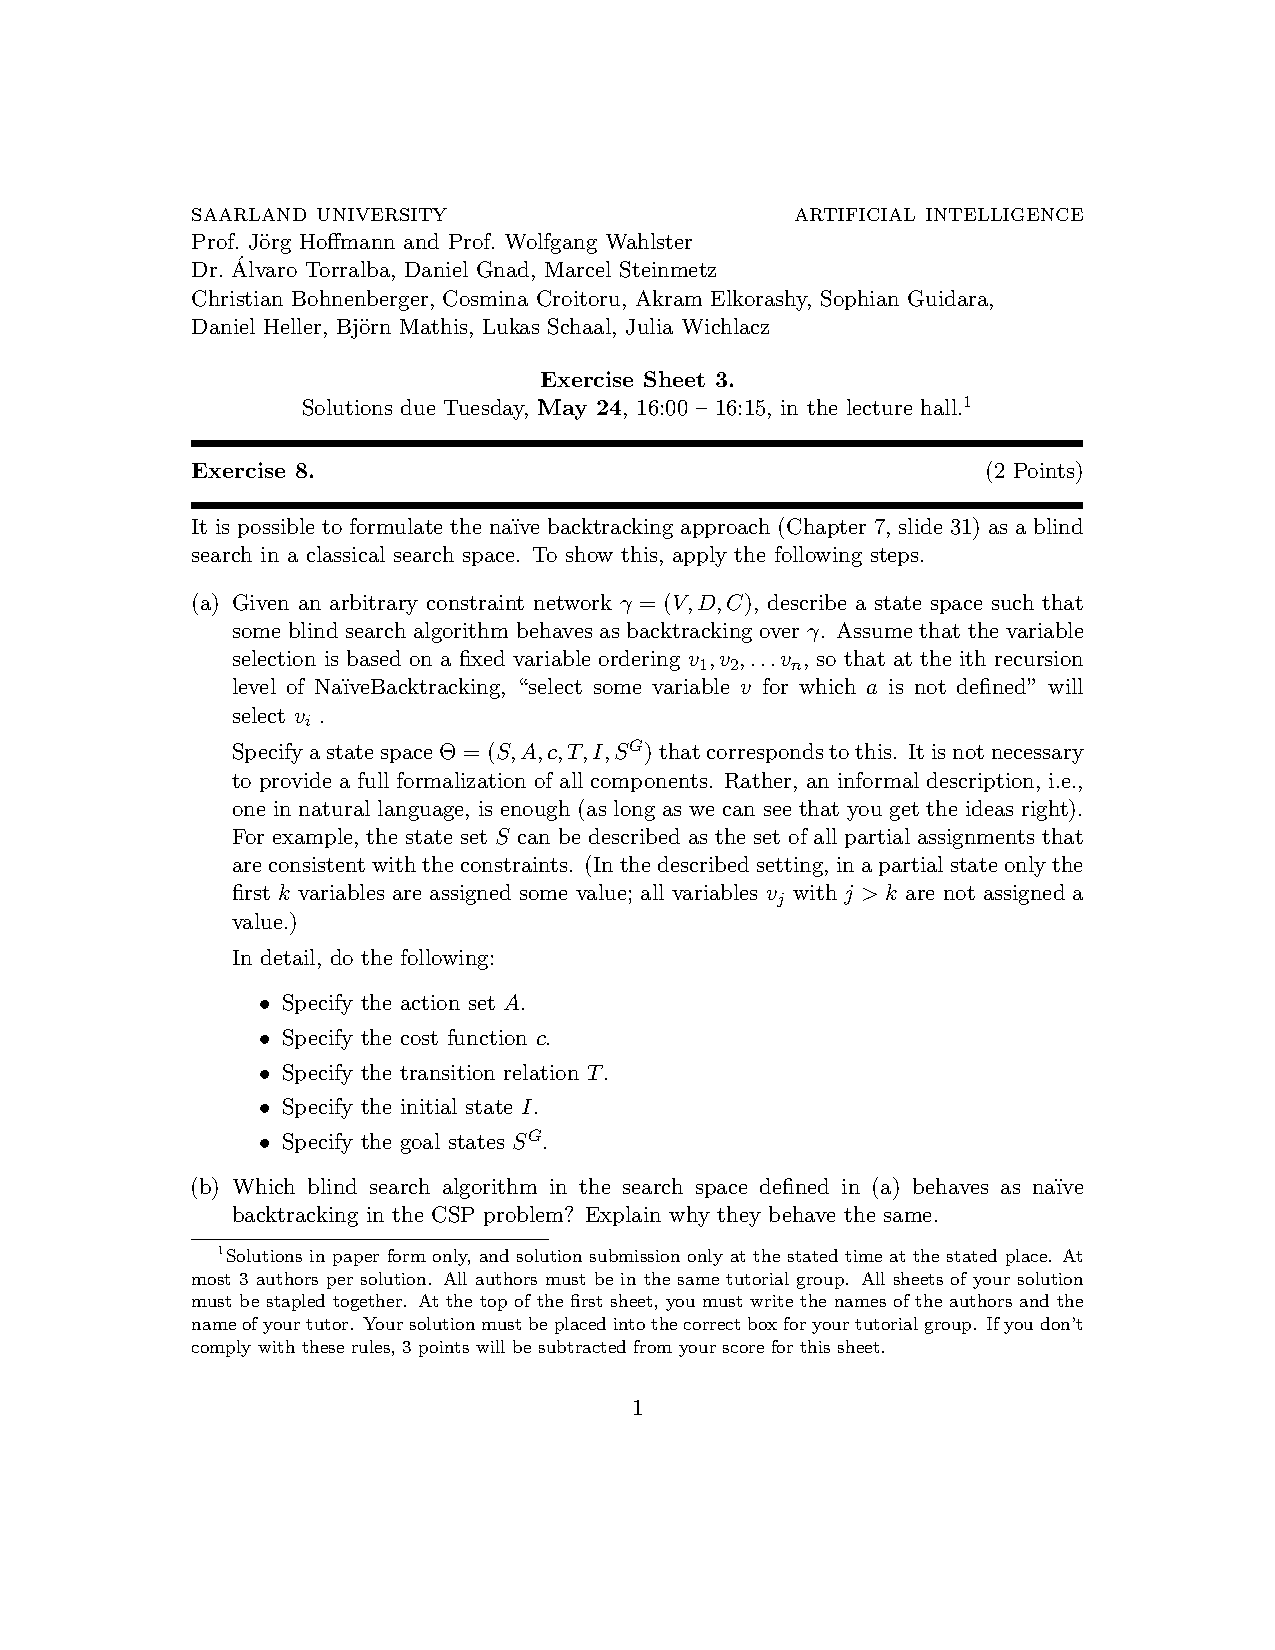
\includepdf[pages=-,nup=2x2]{Old/ai16_sheet03_solution.pdf}
    
    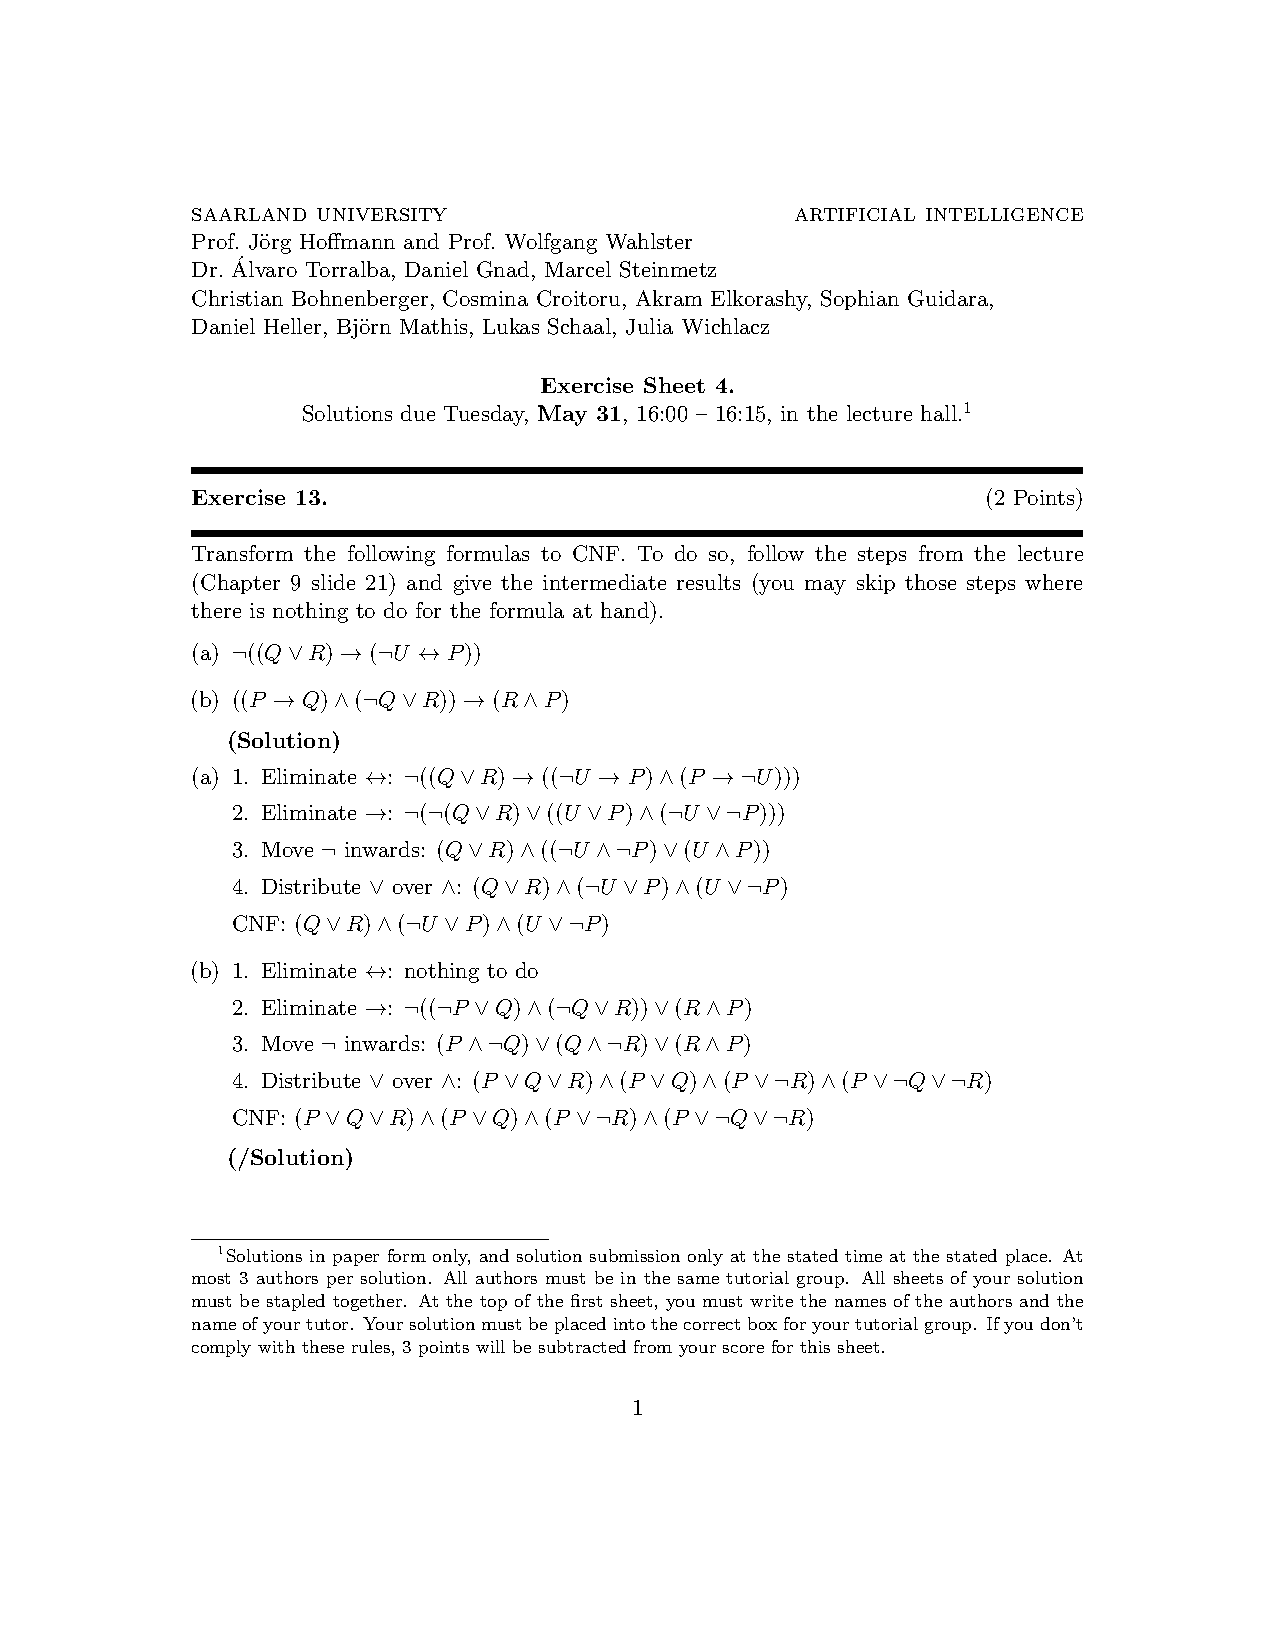
\includepdf[pages=-,nup=2x2]{Old/ai16_sheet04_solution.pdf}
    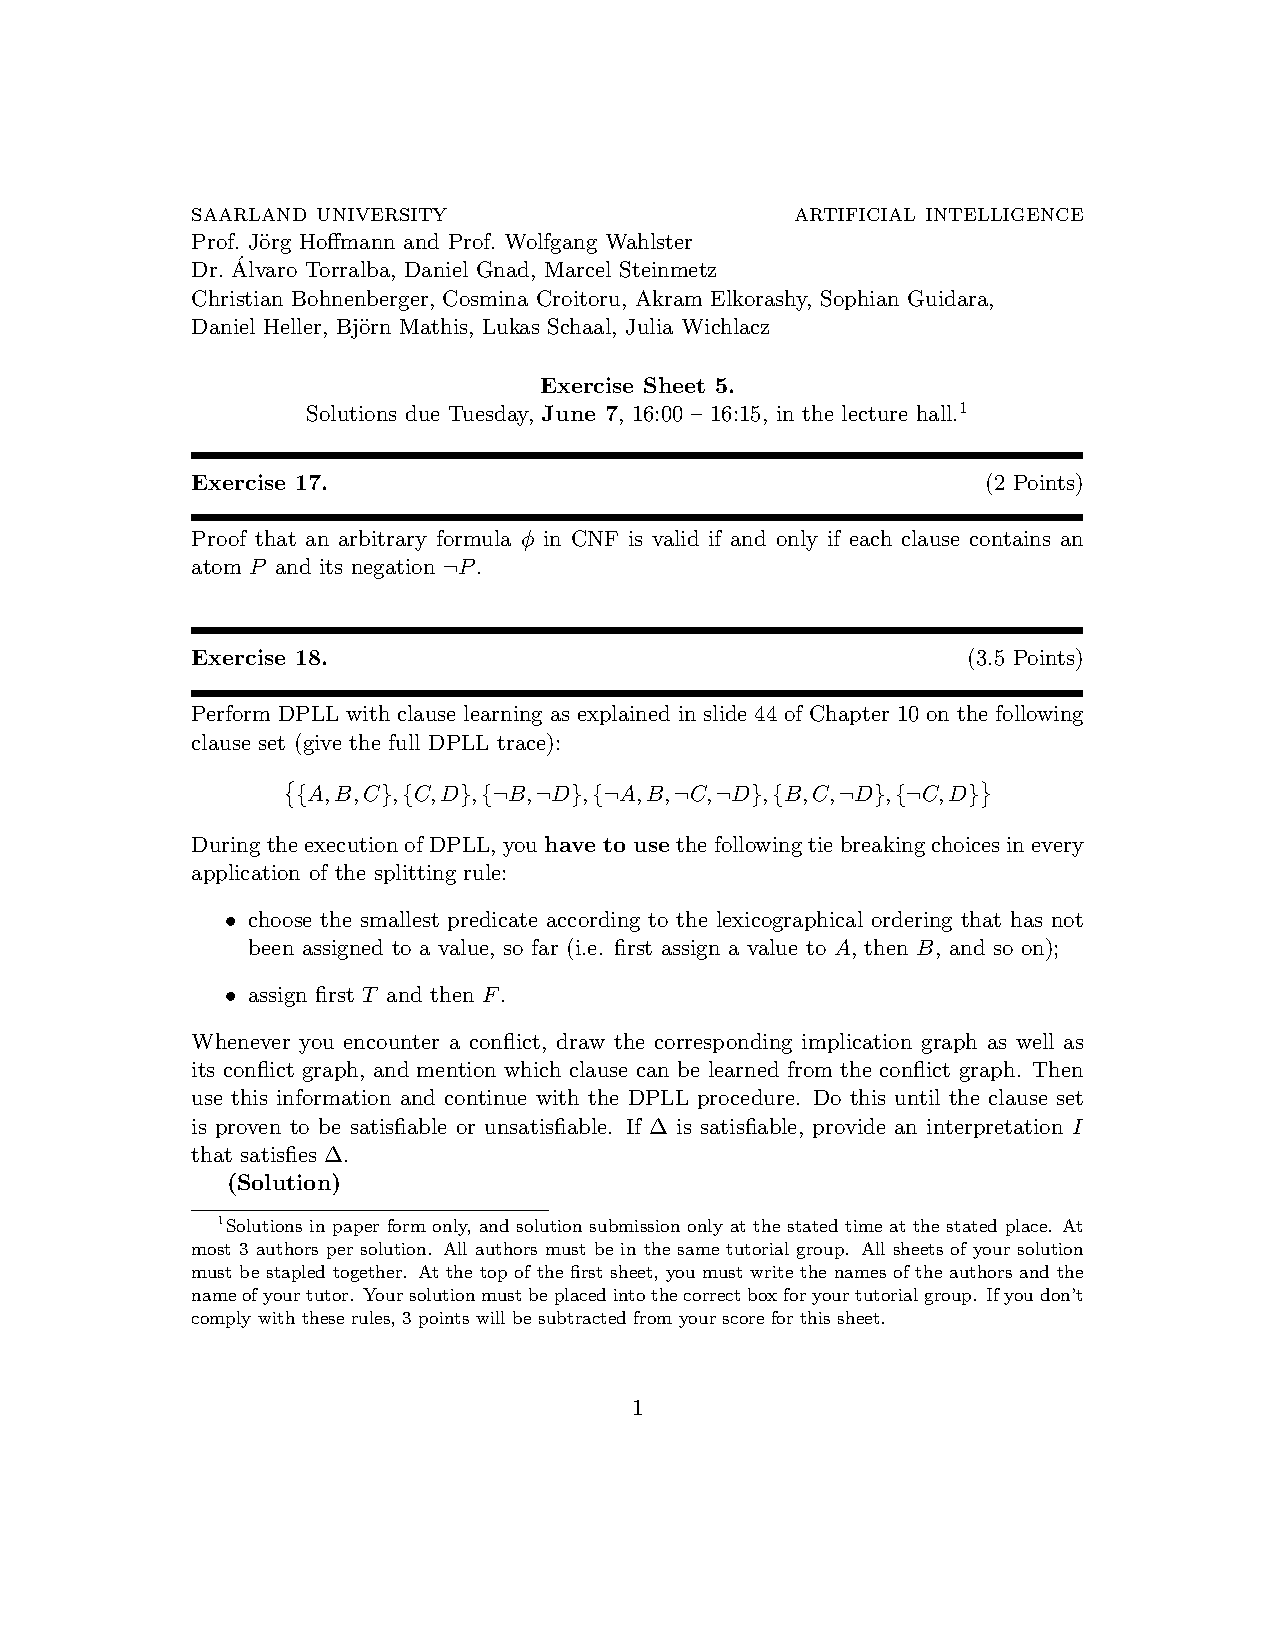
\includepdf[pages=-,nup=2x2]{Old/ai16_sheet05_solution.pdf}
    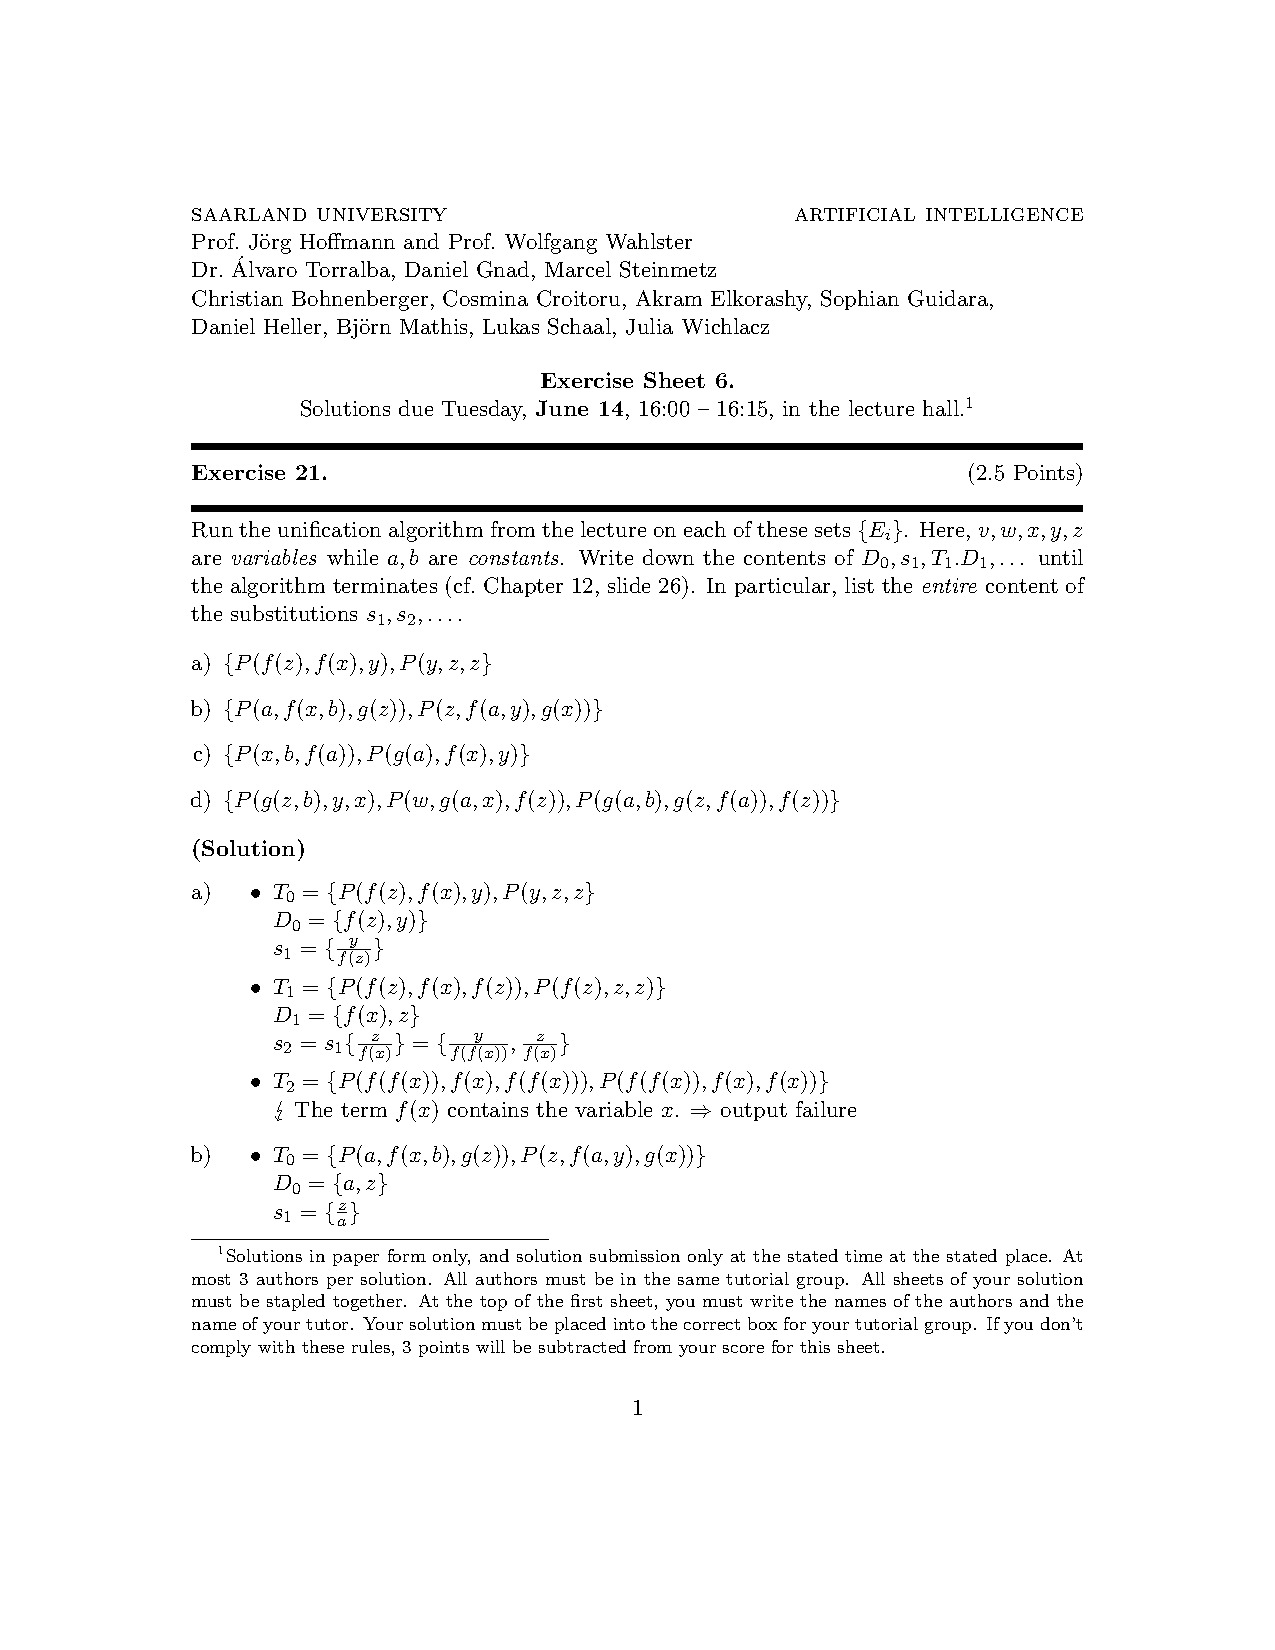
\includepdf[pages=-,nup=2x2]{Old/ai16_sheet06_solution.pdf}
    
    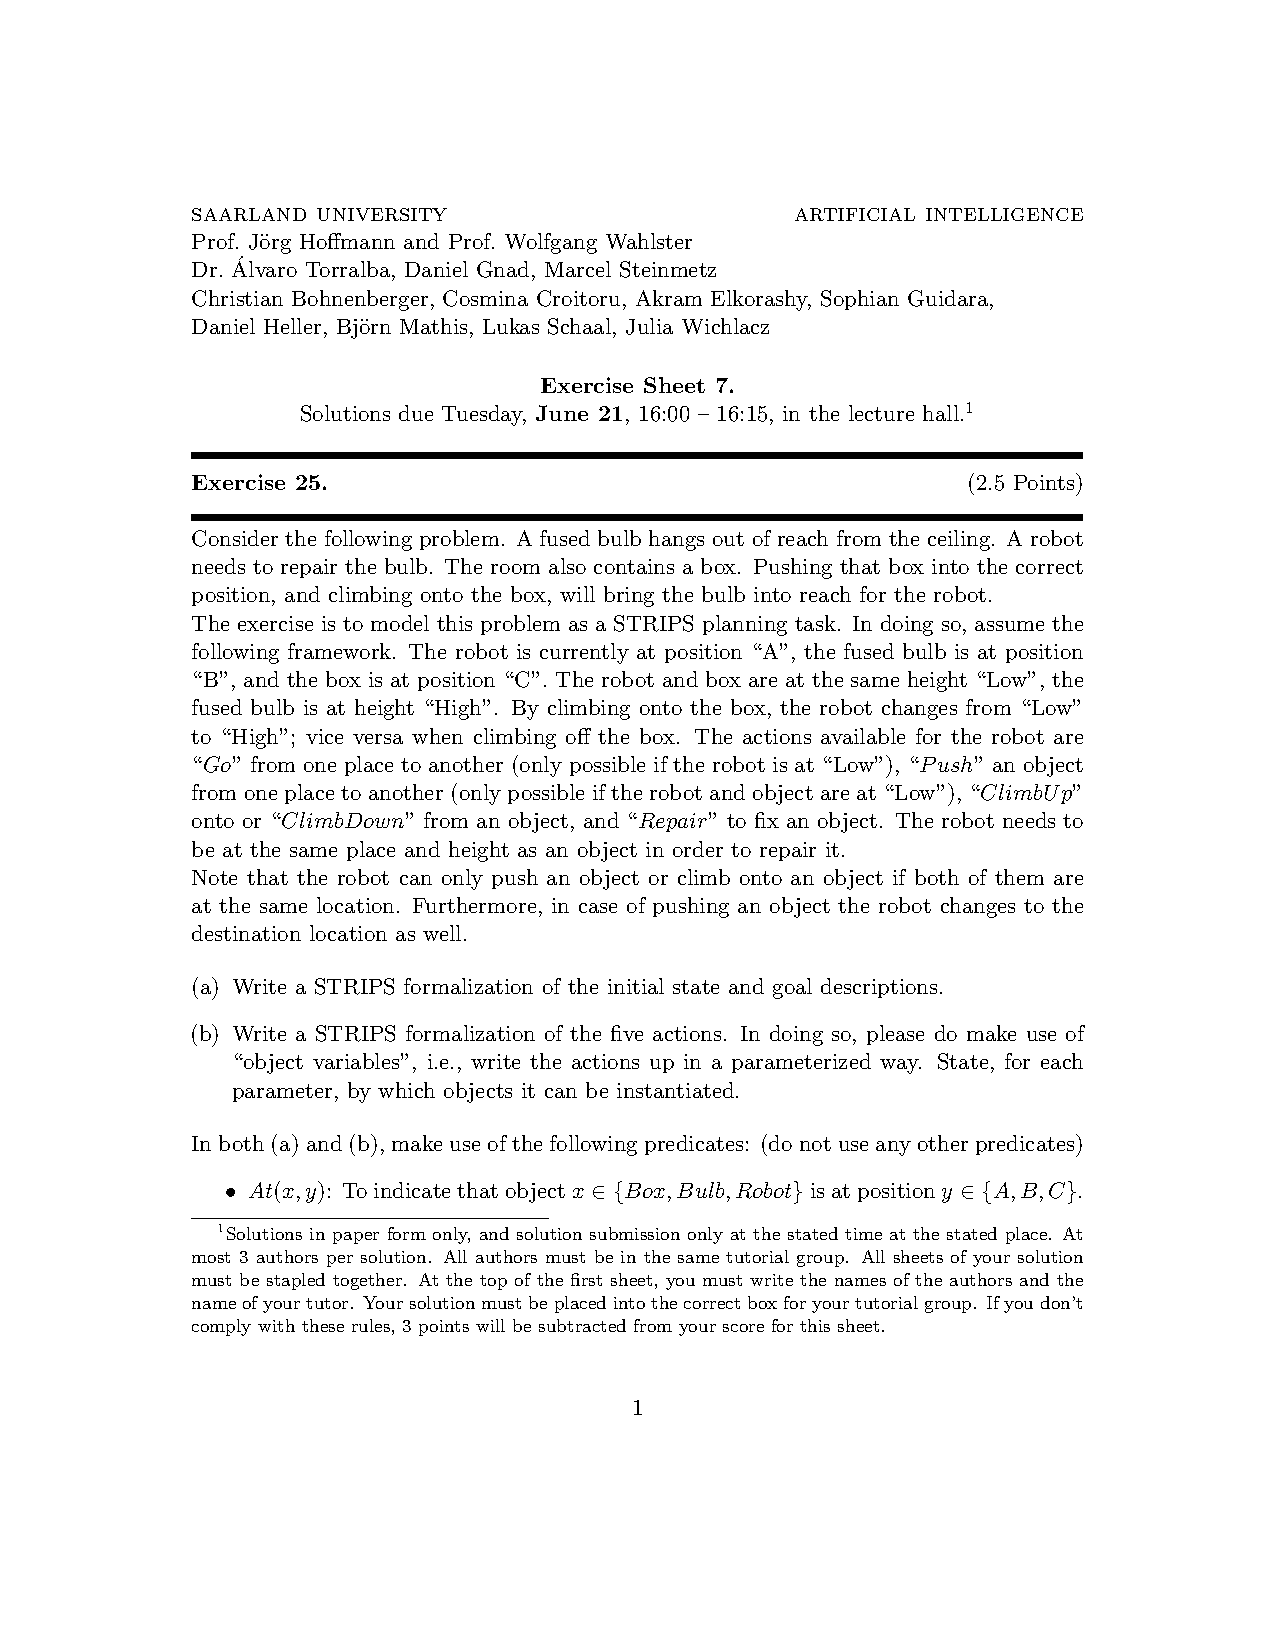
\includepdf[pages=-,nup=2x2]{Old/ai16_sheet07_solution.pdf}
    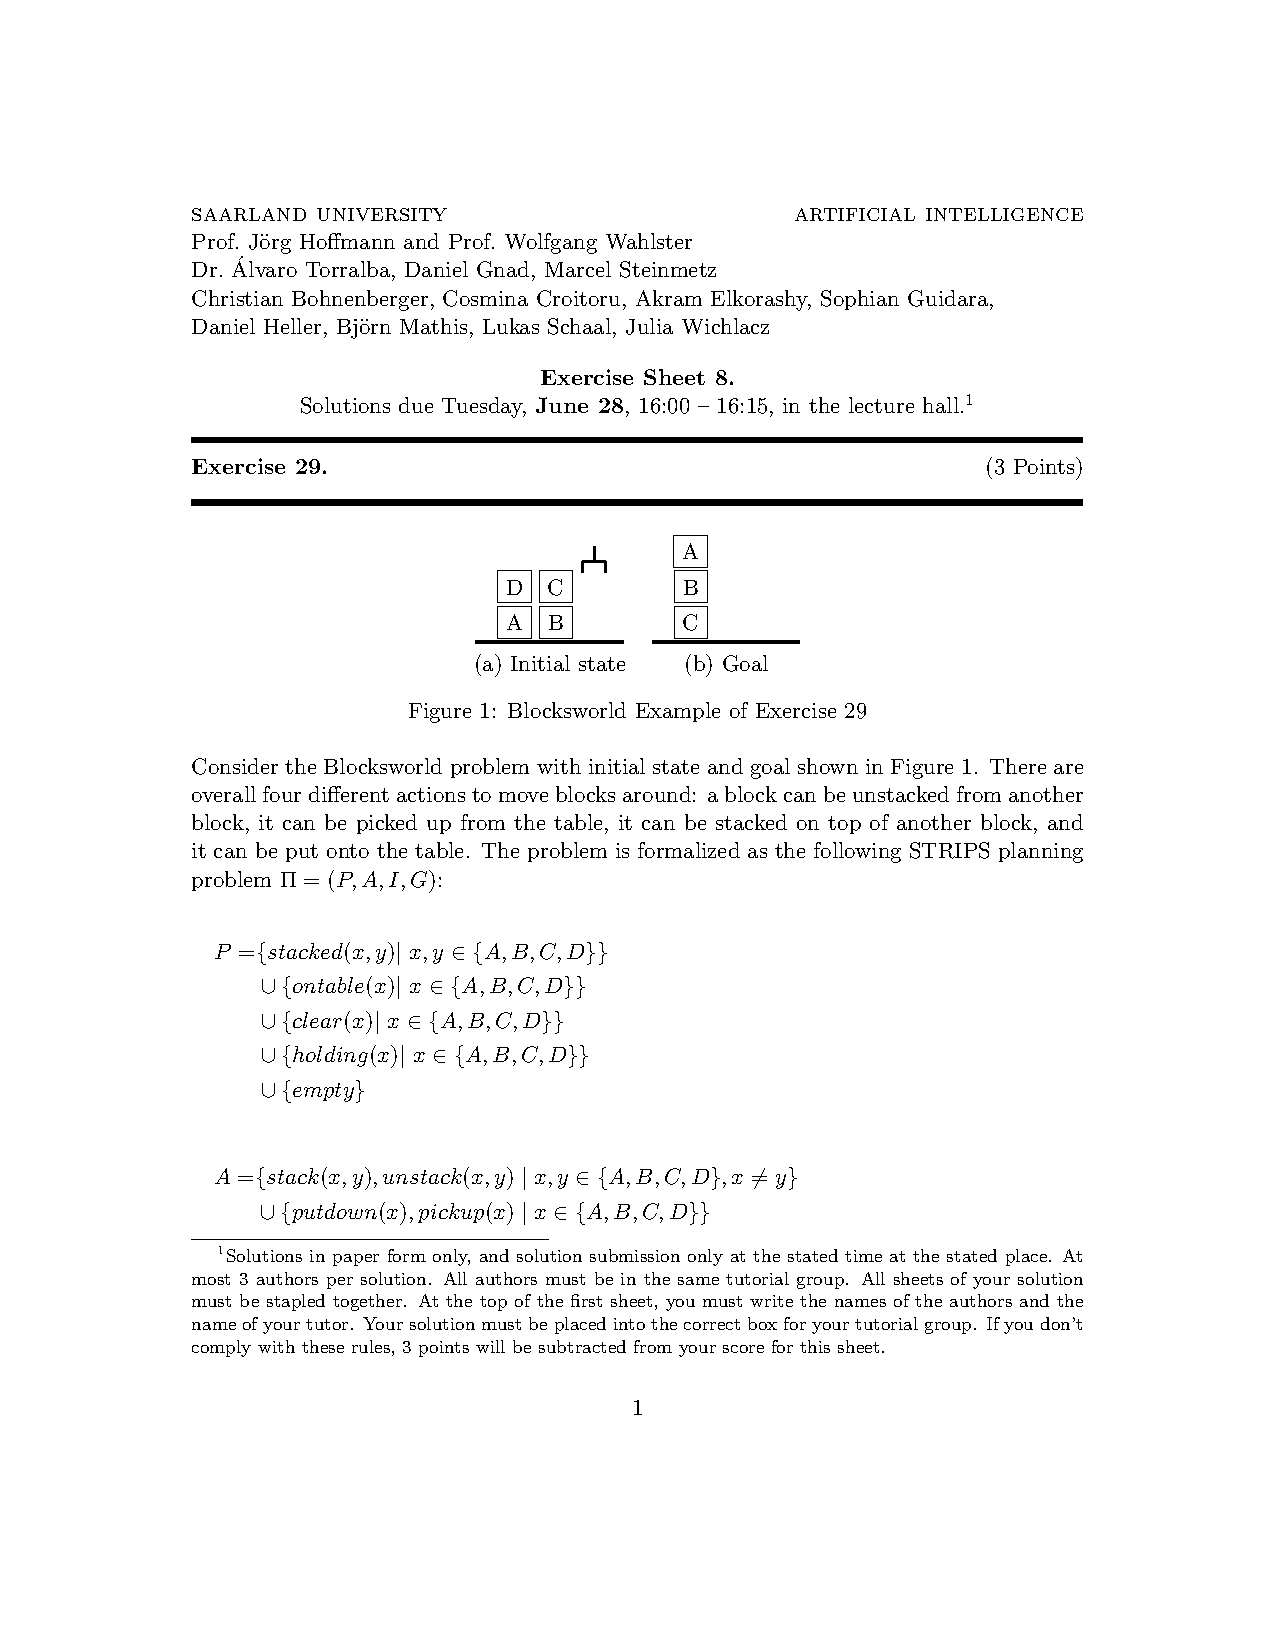
\includepdf[pages=-,nup=2x2]{Old/ai16_sheet08_solution.pdf}
    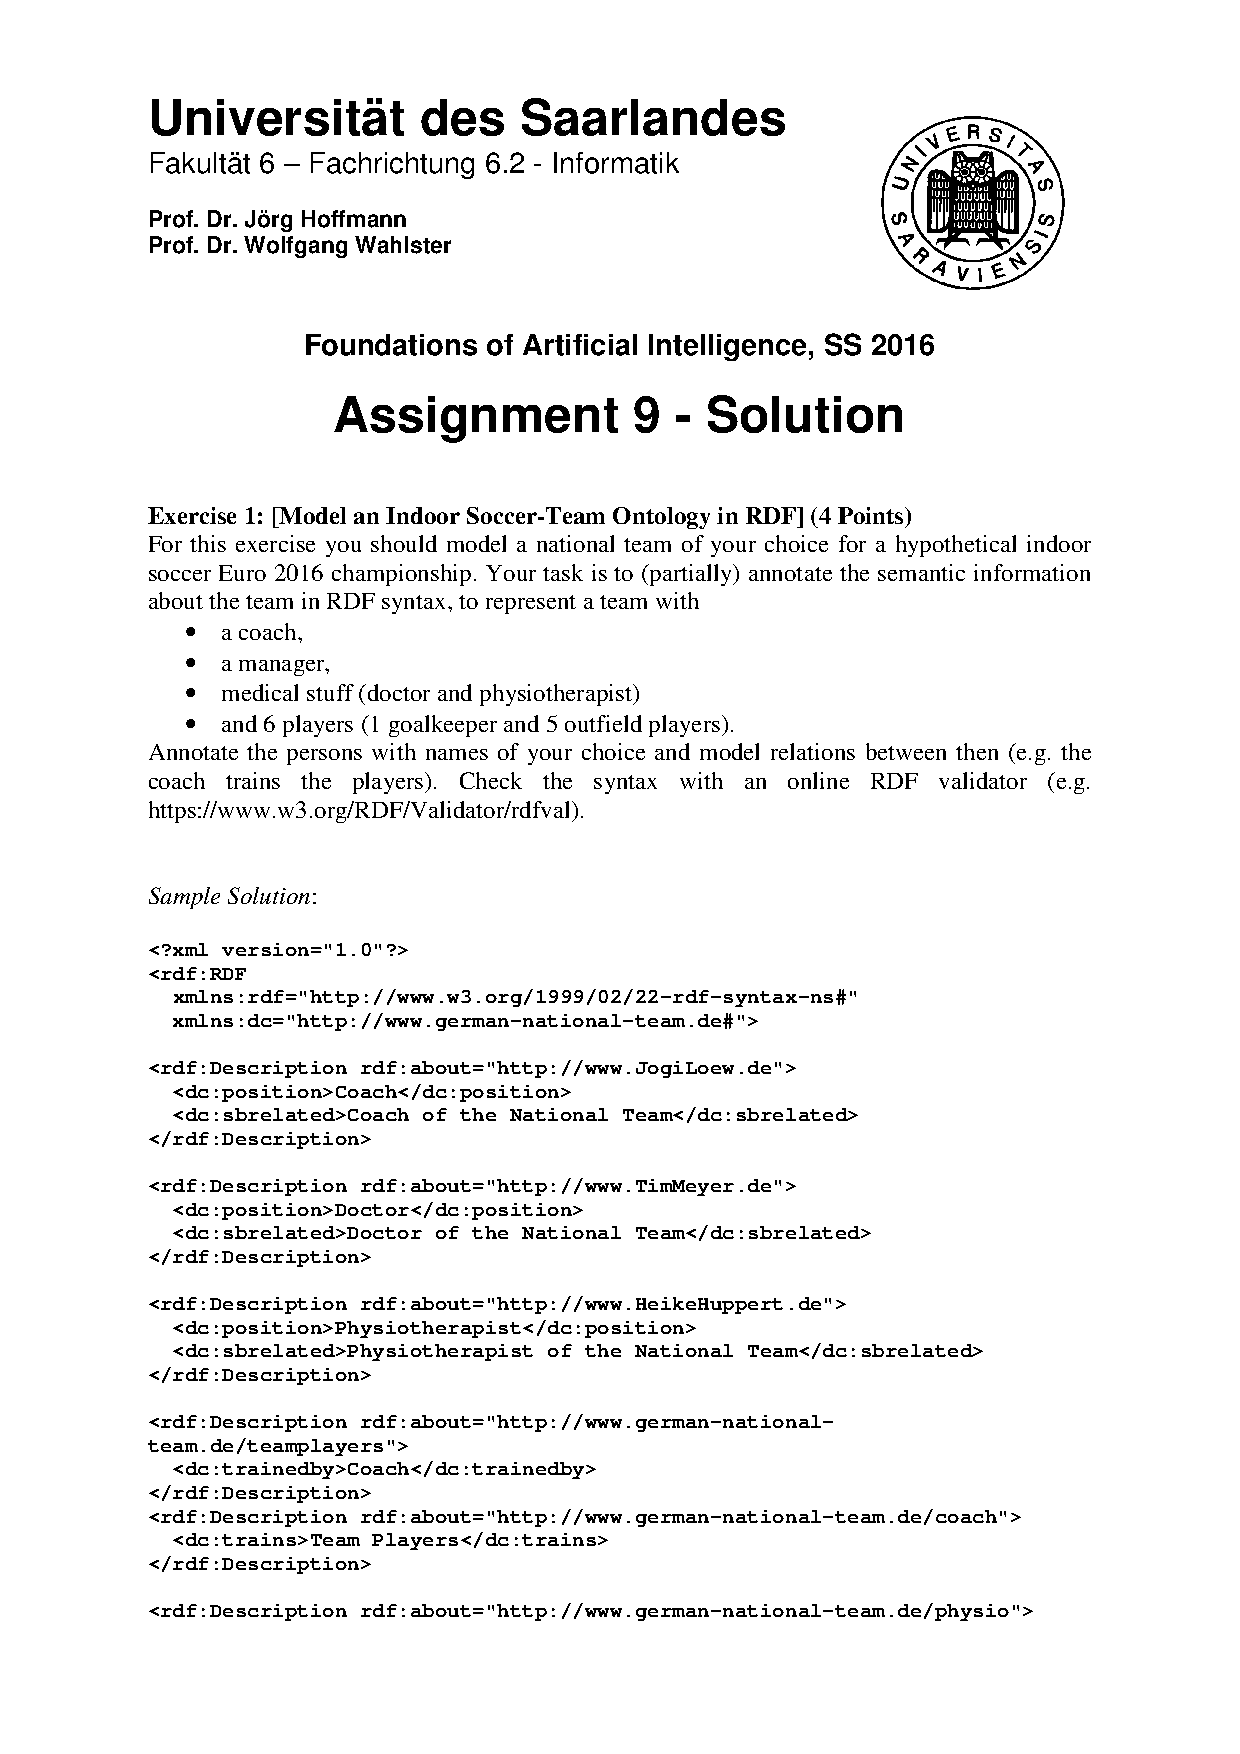
\includepdf[pages=-,nup=2x2]{Old/ai16_sheet09_solution.pdf}
    
    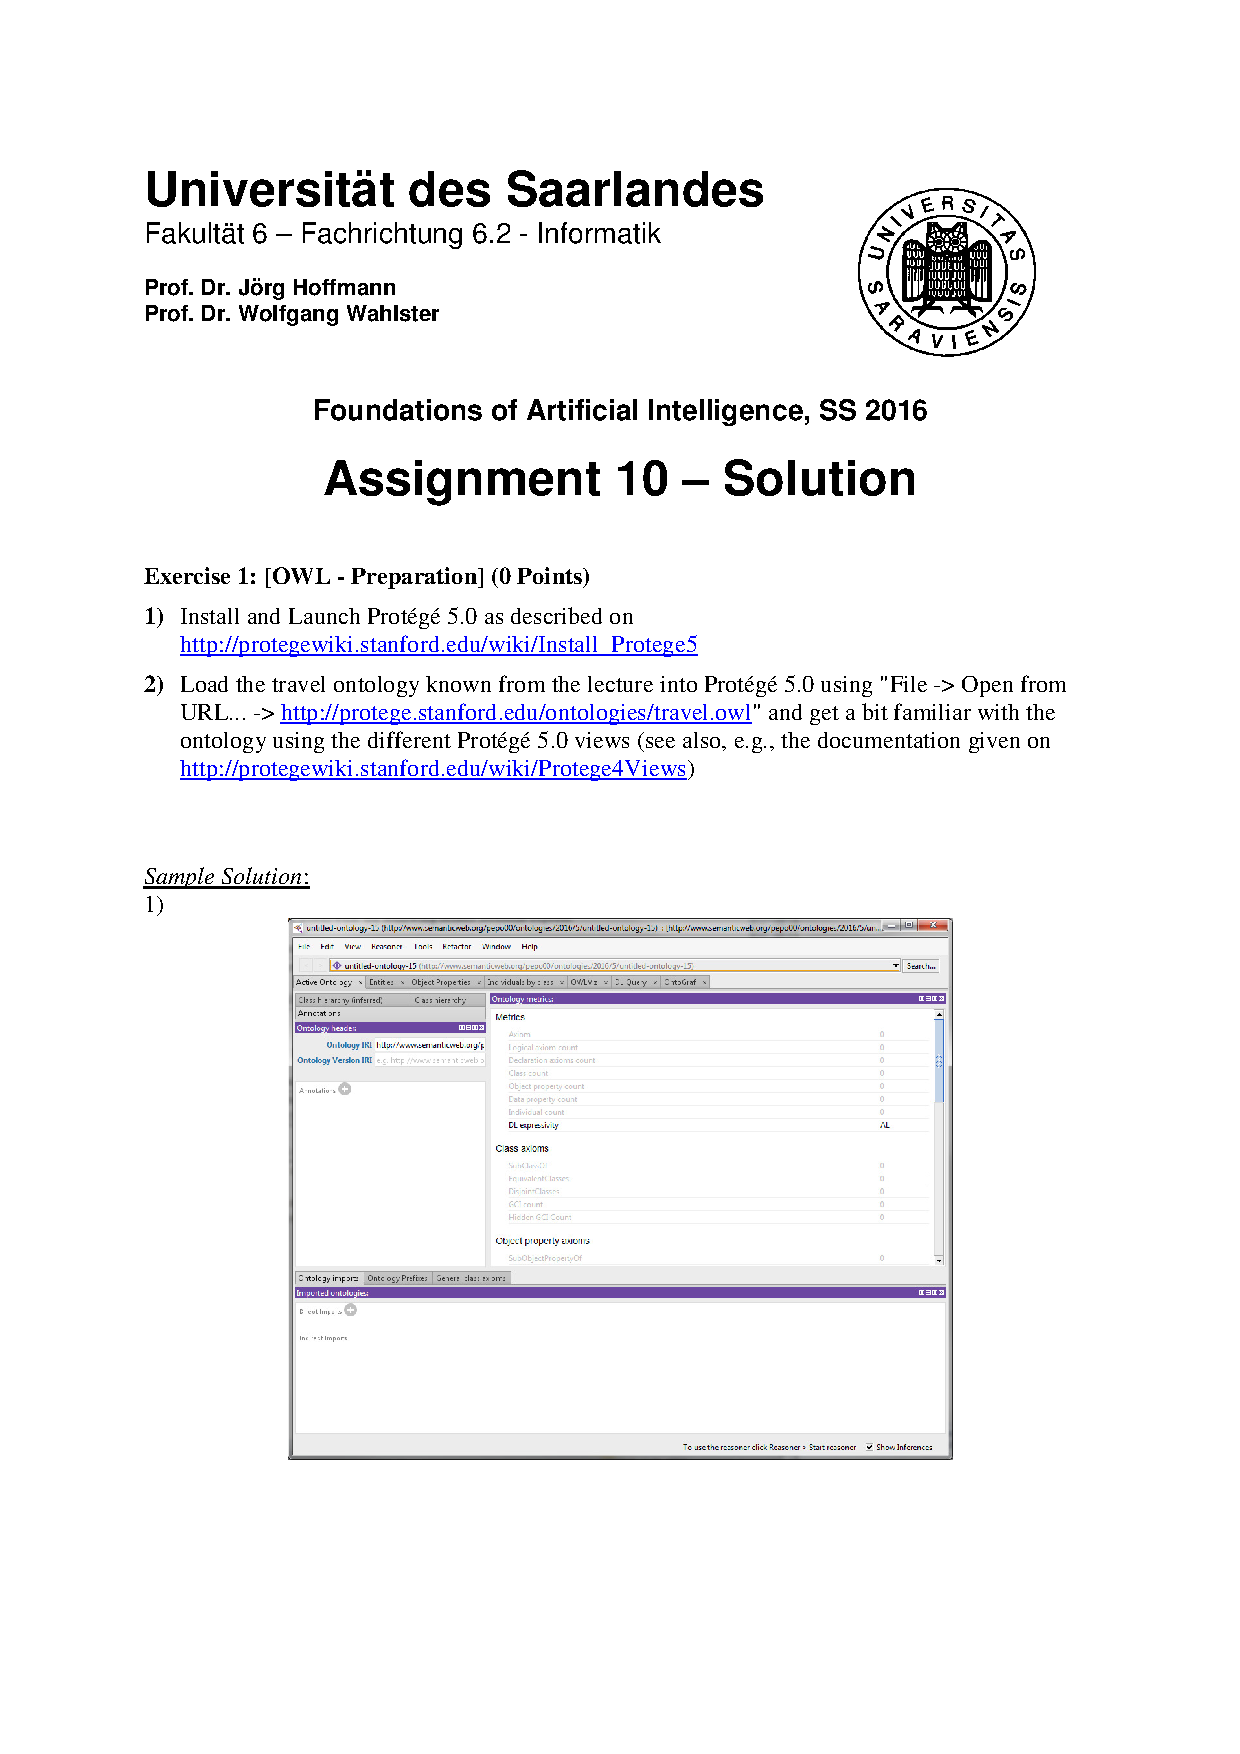
\includepdf[pages=-,nup=2x2]{Old/ai16_sheet10_solution.pdf}
    

\section{Exams}
    
    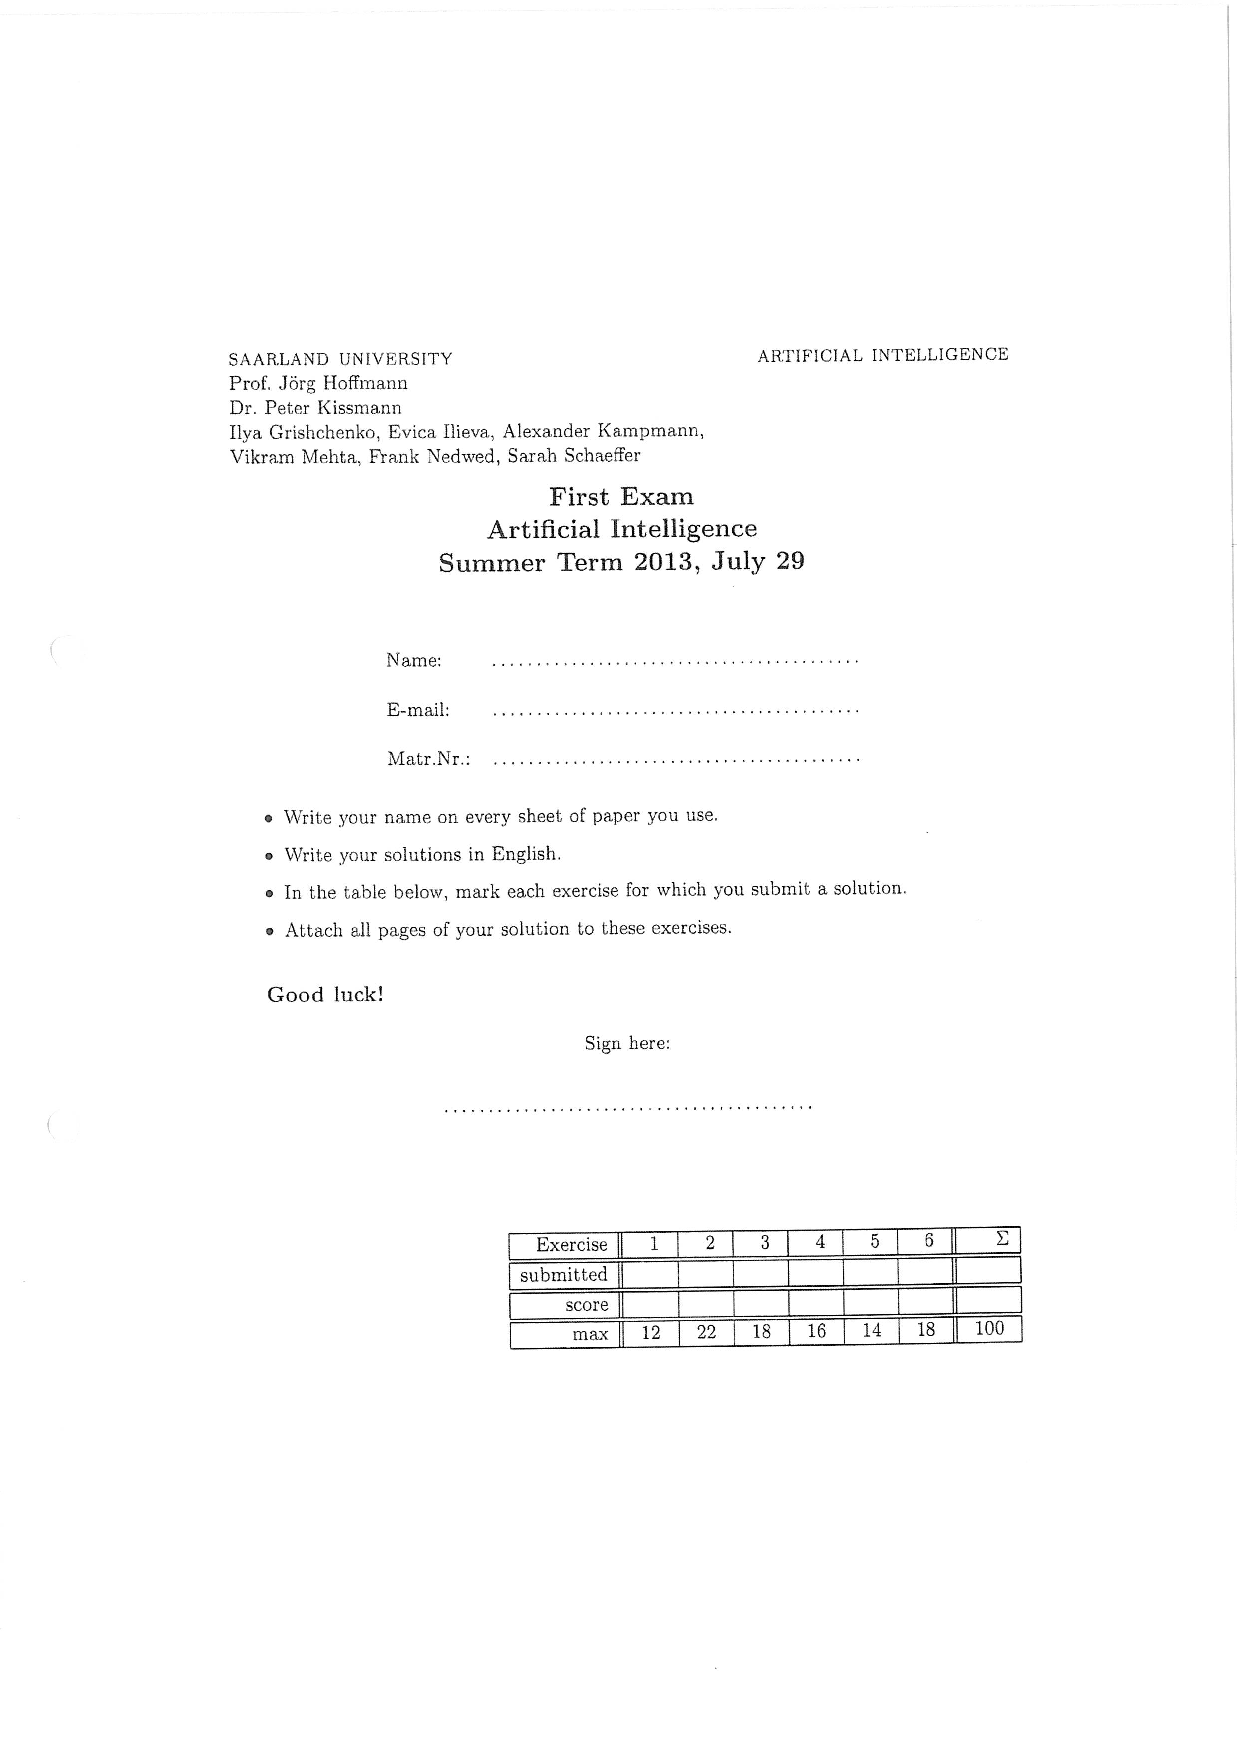
\includepdf[pages=-]{ai_ss13_endterm (1).pdf}
    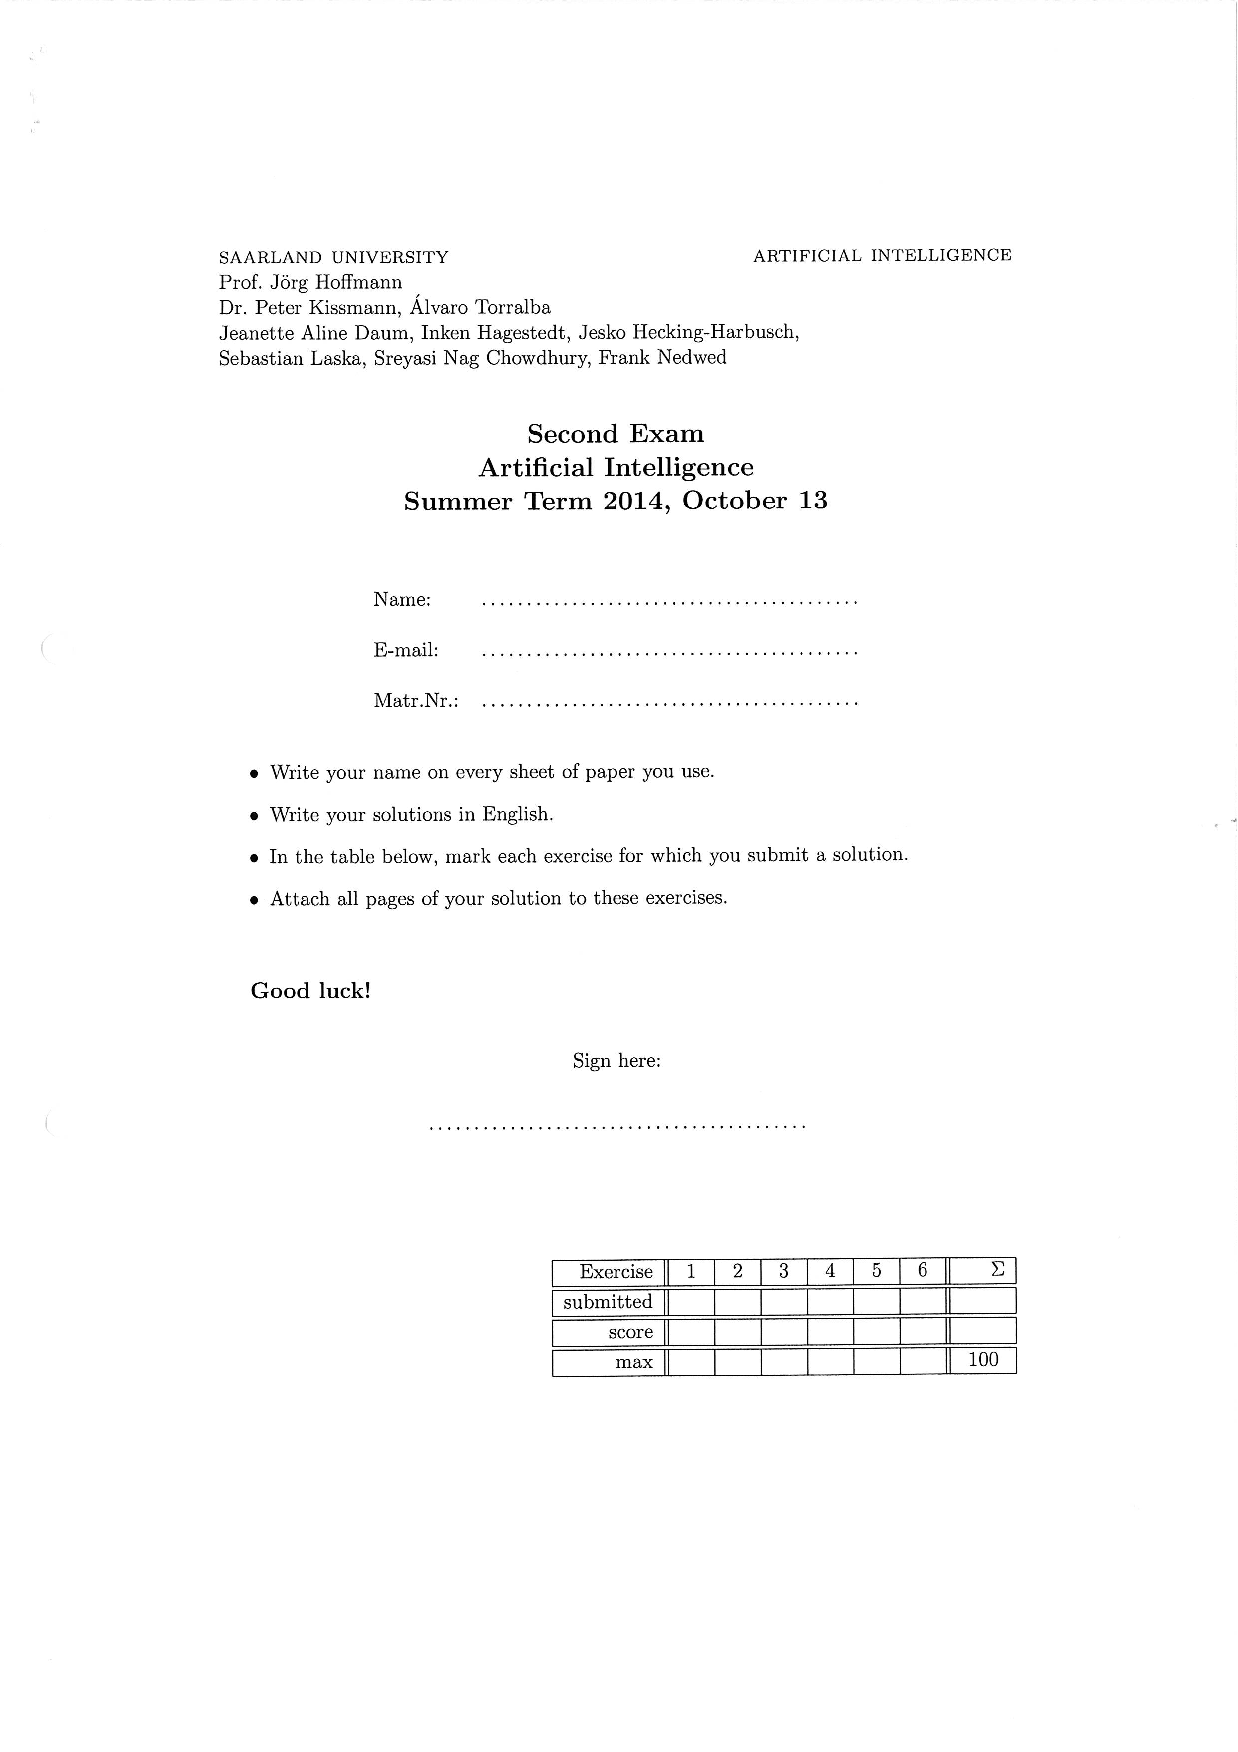
\includepdf[pages=-]{ai_ss14_reexam (1).pdf}
    \includepdf[pages=-]{ai_ss14_reexam_sol (1).pdf}
    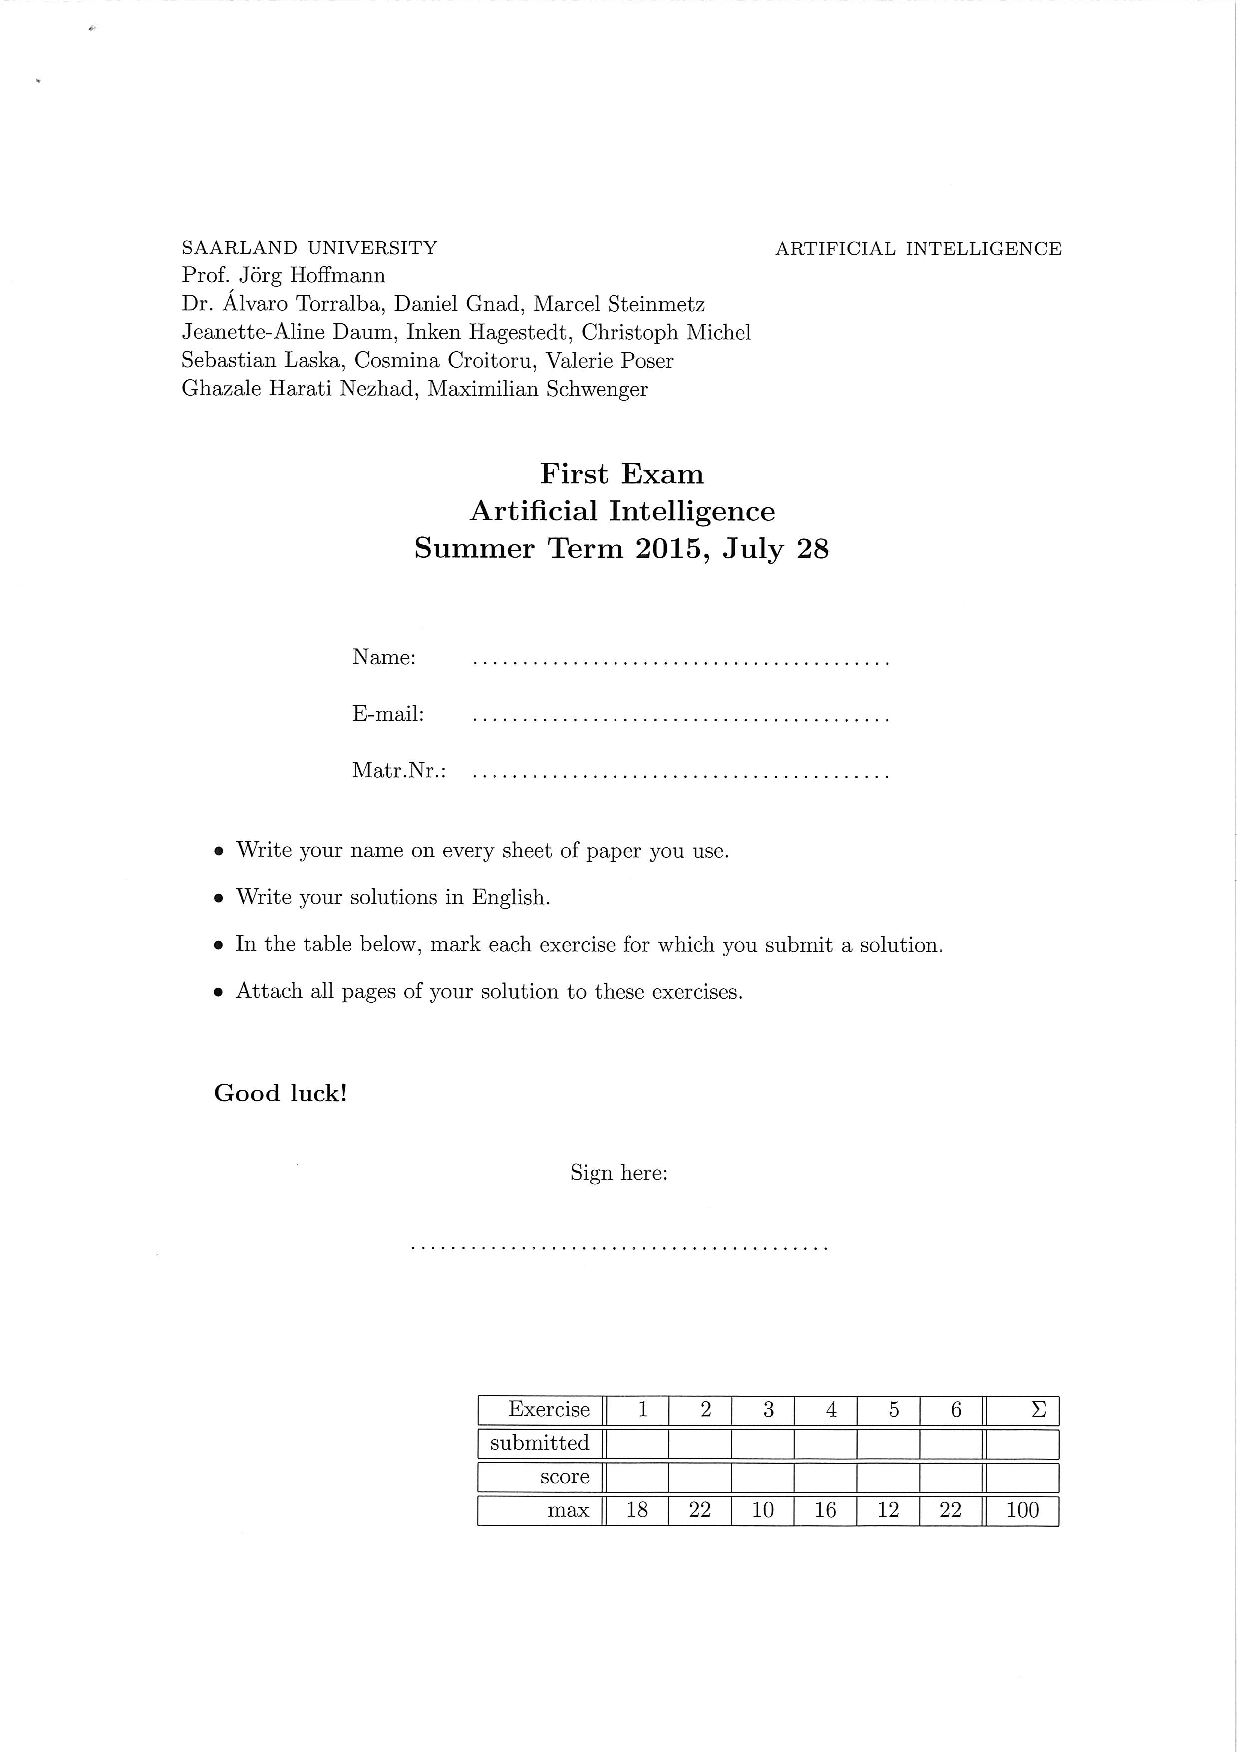
\includepdf[pages=-]{ai_ss15_exam (1).pdf}

\end{document}
